% Overleaf: (1) Upload all .png files in the SAME folder as this .tex (project root).
% (2) Upload refs.bib next to full_report.tex (name must match \\bibliography{refs}).
% (3) Menu -> Compiler = pdfLaTeX. Menu -> Bibliography = BibTeX (not BibLaTeX).
% (4) Recompile 2--3 times after first run so citations and refs resolve.
% !TeX program = pdflatex
% !BIB program = bibtex
\documentclass[conference]{IEEEtran}

\usepackage[T1]{fontenc}
\usepackage{cite}
\usepackage{graphicx}
\usepackage{dblfloatfix}
\usepackage{stfloats}
\usepackage{balance}
\usepackage{url}
\usepackage{hyperref}
\usepackage{booktabs}
\usepackage{tabularx}
\usepackage{array}
\usepackage{enumitem}
\usepackage{listings}
\usepackage{xcolor}
\usepackage{microtype}
\usepackage{colortbl}
\usepackage{tikz}
\usetikzlibrary{arrows.meta,positioning,fit,calc,shapes.geometric}

% Overleaf project root = cwd: keep PNGs beside this file. Extra paths help local git layouts.
\graphicspath{%
  {./}%
  {figures/}%
  {./figures/}%
  {thejes_updates/ieee_full_report/}%
  {./thejes_updates/ieee_full_report/}%
}
% Float placement: keep figures/tables closer to text and reduce vertical whitespace.
\renewcommand{\topfraction}{0.92}
\renewcommand{\textfraction}{0.07}
\renewcommand{\floatpagefraction}{0.85}
\setlength{\textfloatsep}{6pt plus 2pt minus 2pt}
\setlength{\floatsep}{6pt plus 2pt minus 2pt}
\setlength{\intextsep}{8pt plus 4pt minus 2pt}
\setlength{\dbltextfloatsep}{6pt plus 2pt minus 2pt}
\setlength{\dblfloatsep}{6pt plus 2pt minus 2pt}
\setlength{\abovecaptionskip}{4pt}
\setlength{\belowcaptionskip}{0pt}
\renewcommand{\dbltopfraction}{0.92}
\setcounter{dblbotnumber}{2}

\hypersetup{hidelinks}
\sloppy
\emergencystretch=3em
\hyphenpenalty=50
\tolerance=1000

\lstset{
  basicstyle=\ttfamily\footnotesize,
  breaklines=true,
  frame=single,
  columns=fullflexible,
  rulecolor=\color{black!20},
}

\title{WOS Project Report: A Desktop Workspace Orchestrator with Tool-Calling and Fine-Tuned Orchestration Models}

\author{
\centering
{\renewcommand{\arraystretch}{1.08}%
\setlength{\tabcolsep}{6pt}%
% Row 1: three authors
\begin{tabular}{ccc}
Jayam Shah &
Thejes Raj Gangadhar &
Yashwanth Reddy Katipally \\
\textit{Dept of Applied Data Intelligence} &
\textit{Dept of Applied Data Intelligence} &
\textit{Dept of Applied Data Intelligence} \\
\textit{San Jose State University} &
\textit{San Jose State University} &
\textit{San Jose State University} \\
San Jose, CA USA & San Jose, CA USA & San Jose, CA USA \\
\url{jayam.shah@sjsu.edu} &
\url{thejesraj.gangadhar@sjsu.edu} &
\url{yashwanth.katipally@sjsu.edu}%
\end{tabular}}\\[0.9em]
{\renewcommand{\arraystretch}{1.08}%
\setlength{\tabcolsep}{6pt}%
% Row 2: fourth author
\begin{tabular}{c}
Winston Chen \\
\textit{Dept of Applied Data Intelligence} \\
\textit{San Jose State University} \\
San Jose, CA USA \\
\url{winston.chen@sjsu.edu}
\end{tabular}}%
}

\begin{document}
\raggedbottom
\maketitle
\begin{abstract}
Work in modern organizations is distributed across many applications, including chat, issue tracking, source control, calendars, email, and internal systems. This fragmentation forces users to manually search multiple locations, reconcile partial context, and repeatedly translate intent into actions across different interfaces. WOS centralizes this workflow by providing an agentic interface that can retrieve information and execute actions through structured tool calls while preserving conversation state and traceability. In addition to reliability, a practical deployment constraint is cost: continuous reliance on large hosted models can be prohibitive for high-frequency, tool-heavy workflows. WOS addresses both by combining a contract-enforcing execution harness with orchestration fine-tuning on schema-aligned tool-use trajectories. Fine-tuning enables smaller or self-hosted backends to follow the same serving contract, reducing per-request cost while preserving contract-level tool-use behavior.
\end{abstract}
\section{Introduction}
\subsection{Project Background and Executive Summary}
Modern knowledge work is executed across a growing number of disconnected applications, including chat platforms, issue trackers, source control systems, calendars, email, document stores, and internal dashboards. This fragmentation creates an operational bottleneck: users must repeatedly switch contexts, search multiple locations, reconcile partial information, and manually transfer content between systems. In practice, the overhead of context switching and information retrieval becomes a limiting factor in both individual productivity and team coordination, especially when tasks span several tools (e.g., “find the relevant Slack thread, locate the matching Jira ticket, identify the related pull request, and summarize the status for stakeholders”).

WOS (WorkOS) is a desktop application designed to unify these workflows into a single agentic interface. Our targeted problem is that workspace applications are “far and many,” and completing a single task often requires checking multiple places. WOS addresses this by integrating external workspace services into one tool-enabled assistant surface, conceptually similar to the direction taken by Cursor-like products that combine codebase context with agentic tool execution. Instead of requiring the user to manually traverse each application, WOS provides an orchestrator that can query services, run tool calls, and present synthesized outputs while preserving traceability of what sources were used.

From an implementation perspective, WOS is structured as an Electron desktop application. The renderer provides a unified user interface for chat and configuration, while the Electron main process performs orchestration: it builds a system prompt, selects a model provider, streams outputs, executes structured tool calls, and persists conversations. Because real-world orchestration quality depends on tool-use reliability, orchestration behavior is improved through fine-tuning on contract-aligned tool trajectories. Finally, to support flexible deployment, WOS can use both hosted APIs and self-hosted serving backends, such as Hugging Face Spaces, AWS, or RunPod.

We planned and executed the development of WOS across four concurrent tracks: (i) the application harness---Electron desktop client, IPC layer, SQLite persistence, streaming protocol, and provider abstraction; (ii) the feature modules---a Projects workspace for AI-powered project management, a Meetings intelligence tab for transcript analysis and calendar integration, an Automations engine for schedule and event-driven workflows, and an Apps/MCP integration marketplace for connecting external services and Model Context Protocol servers; (iii) model development---orchestration data engineering, fine-tuning on strict tool-use trajectories, and deployment of the resulting checkpoint on a Hugging Face Space backed by a vLLM inference server; and (iv) system evaluation and audit, validating orchestration correctness and end-to-end workflow behavior.

The primary contribution of WOS is a complete, production-oriented desktop workspace orchestrator with a rich set of domain-specific modules that address the real operational costs of fragmented knowledge work. Secondary contributions include a reproducible fine-tuning pipeline for tool-use orchestration, a provider abstraction that supports swappable model backends (OpenAI, Anthropic, or self-hosted vLLM), and a Hugging Face Space deployment path that delivers a fine-tuned orchestration model without modifying the application's runtime contract.

\subsection{Project Requirements}
Requirements for the agentic workspace orchestrator are specified across four observable and measurable domains: functional integration, artificial intelligence (AI) behavior, data management, and operational performance.

Functional integration requires the system to connect with supported workspace applications, execute information retrieval operations via strict tool calls, modify or create external artifacts under explicit authorization, and maintain a persistent conversational state to support iterative user workflows. These requirements are verified through scripted integration tests that assert the successful execution of targeted tool calls and the verifiable presence of the resulting artifacts in isolated mock environments.

AI-powered behavioral requirements mandate that the orchestrator produce syntactically valid and semantically aligned tool calls. This is quantified by a tool-call correctness rate, demanding perfection for schema compliance and registry alignment. Furthermore, the system must exhibit robust recovery behaviors; upon receiving execution errors, the agent must autonomously correct the parameters or trigger a formal clarification mechanism. Recovery success is evaluated against a deterministic suite of failure-injection scenarios.

Data requirements dictate the use of strict, multi-turn trajectories characterized by canonical role ordering and explicit pairing of tool calls with corresponding results. Data integrity is enforced via automated validation scripts that reject malformed records, ensuring strict deterministic partitioning (train, validation, and blind-test sets) to eliminate evaluation leakage.

Operational and performance requirements constrain the system's runtime latency and resource footprint. Measurable thresholds include time-to-first-token during streaming and end-to-end task completion times, ensuring responsive interactive performance while preventing context overflow through active token-budget management.

Application feature requirements span four primary modules. The \textbf{Projects module} must support creating, reading, updating, and deleting project records; linking external resources from connected services (Slack channels, GitHub repositories, Jira projects, Google Drive folders); generating AI-powered project health scores and risk signals by querying linked resources; displaying a timestamped activity feed and people roster; surfacing pinned notes, custom widgets, and recorded decisions; and exporting project summaries in JSON, Markdown, and HTML formats. The \textbf{Meetings module} must retrieve events from connected Google Calendar accounts, discover and process Google Drive meeting recordings, accept locally uploaded audio files for offline transcription, extract structured action items and decisions through AI analysis, and deliver results to connected Slack workspaces or email. The \textbf{Automations module} must persist automation definitions with cron-based schedules, event hooks (triggered by application events), and outbound webhooks with an optionally tunneled local HTTP endpoint; execute automations on schedule or on demand; support dry-run simulation of automation logic before live execution; and maintain a timestamped per-run audit log. The \textbf{Apps and MCP module} must present a first-party integration marketplace, execute OAuth 2.0 authorization flows for Slack, GitHub, Jira, and Google, manage API key credentials for custom services, enumerate and connect Model Context Protocol servers via \texttt{stdio} or HTTP transport, and expose MCP server tools through the tool registry with sanitized, schema-valid names.

Orchestration quality requirements for AI-powered features mandate that the agent correctly invoke tools to satisfy per-tab workflows (e.g., AI project summarization invokes the correct tool with the correct project identifier), that the \texttt{AskUser} clarification mechanism fires when required parameters are missing, and that the intent engine correctly pre-filters irrelevant tool families to remain within context-window budget. Data requirements include maintaining strict role-sequence integrity in conversation history, enforcing workspace path boundaries for file-accessing tools (\texttt{validatePath}), and encrypting all stored service credentials at rest.

\subsection{Project Deliverables}
WOS deliverables are treated as a portfolio of artifacts that can be independently validated.

The \textbf{primary deliverable} is the WOS desktop application: a full-featured Electron application comprising a React/TypeScript UI with five navigation areas (Chat, Projects, Meetings, Automations, Apps/MCP), a SQLite persistence layer for conversations, projects, automations, and tool-call traces, a provider abstraction for multiple LLM backends, a dynamic tool registry connecting to Slack, GitHub, Jira, and Google, and runtime mechanisms including an intent engine, context compaction, sub-agent routing, a permission store, and encrypted credential management. Additional productivity features include a global command palette with fuzzy search (Cmd/Ctrl+K), voice dictation via an AudioWorklet PCM pipeline, multi-format file attachments, a Debug Drawer for live agent-event observability, and an AI-powered automation authoring wizard (\texttt{parseDescription}).

The \textbf{second deliverable} is the fine-tuned orchestration model: a Qwen-family model trained on schema-aligned multi-turn tool-use trajectories and deployed on a Hugging Face Docker Space with a vLLM inference backend. It is accessible through the application's provider abstraction as a self-hosted, cost-efficient alternative to commercial API providers.

The \textbf{third deliverable} is the orchestration data pipeline: Python scripts and Colab notebooks (\texttt{wos\_orchestration\_colab\_2\_2.ipynb}) that generate, audit, repair, and partition trajectory-structured fine-tuning datasets under strict schema contracts, including deterministic scenario-disjoint train/validation/blind-test splits.

Supplementary deliverables include the curated specialist datasets (meeting summarization and coding instruction), the Playwright end-to-end test suite covering core application workflows, specialist model evaluation results (HumanEval/MBPP and ROUGE), and dataset artifacts linked in the Appendix for reproducibility.
\subsection{Technology and Solution Survey}
Across the last years, the technology landscape relevant to WOS converged around a common thesis: as LLMs became capable of multi-step reasoning, the dominant constraint in real deployments shifted from “can the model speak plausibly” to “can the system safely and reliably act across many tools and contexts.” This shift produced three practical design patterns that directly informed WOS: (i) agentic “single-surface” work environments that unify context and action, (ii) standardized protocols for connecting agents to external tools and resources without prompt bloat, and (iii) deployable inference stacks that preserve a stable, tool-capable API for swapping model backends.

The first pattern is visible in modern AI workbenches such as Cursor and GitHub Copilot, which increasingly emphasize end-to-end task execution rather than isolated completion. Cursor’s agent tooling and documentation describe an environment in which an agent can read a codebase, search, edit, and run commands while being guided by explicit instructions and tool access—an interaction model that strongly resembles WOS’s orchestrator harness, even when WOS targets general workspace apps rather than only code~\cite{cursor_tools}. GitHub Copilot is similarly positioned as a development assistant integrated into the developer workflow, reflecting the broader movement toward “embedded AI” rather than separate chat applications~\cite{copilot_feature}. In this category, the primary architectural differentiator is not the UI but the harness: how the system binds user context, tool access, and a persistent state store to an LLM that streams intermediate reasoning and actions.

The second pattern is tool interoperability. As tool catalogs grow, it becomes counterproductive to paste long tool schemas into the prompt; modern systems instead use standardized interfaces that support tool discovery, selective exposure, and secure execution. The Model Context Protocol (MCP) formalizes a host–client–server design for exposing tools and resources through a JSON-RPC interface, including capability negotiation and authorization mechanisms~\cite{mcp_spec}. Cursor’s documentation explicitly discusses MCP integration as a way to connect external tools to the agent~\cite{cursor_mcp}. For WOS, MCP-style modularity is directly relevant to scalability: it provides a path to integrate many applications without a monolithic prompt and without rewriting core orchestration logic for each tool family.

The third pattern is deployable inference with stable APIs. In practice, application teams often need to switch between hosted providers (for quality) and self-hosted endpoints (for cost, privacy, or custom fine-tunes). OpenAI-style Chat Completions interfaces have become an interoperability layer for this. vLLM provides an OpenAI-compatible API server and explicitly configurable tool-calling support~\cite{vllm_openai_server,vllm_tool_calling}. Hugging Face Docker Spaces provides a container substrate for hosting such servers with configurable ports and runtime variables~\cite{hf_docker_spaces}. WOS’s provider abstraction is aligned with this pattern: provider choice is treated as an implementation detail, while tool calling and orchestration policy remain stable.

Fine-tuning is a method that sits orthogonally to these system patterns but is essential to making them reliable. Tool-capable models exist, yet base behaviors are typically not sufficiently consistent for production orchestration requirements: argument schemas must be respected, tool-call boundaries must be unambiguous, and recovery must be systematic under tool errors and missing inputs. The broader ecosystem has addressed this with structured-output methods and strict schema adherence mechanisms; OpenAI’s “Structured Outputs” describes a design goal of reliably constraining model output to a developer-specified schema, reflecting the same reliability objective that WOS enforces through strict dataset audits and repair steps~\cite{openai_structured_outputs}. WOS’s chosen approach—generate strict tool-use trajectories, validate/repair them, split deterministically, and fine-tune—fits the dominant practice for converting a general model into a contract-following orchestrator.

In parallel, academic work has increasingly treated tool use as a benchmarkable capability rather than an anecdotal demo. API-centric benchmarks and datasets such as API-Bank and Gorilla’s APIBench evaluate whether models can generate correct tool calls and arguments under explicit interfaces~\cite{li-etal-2023-api,patil2023gorilla}. ToolBench/ToolLLM further scales this direction by constructing large collections of real-world APIs and evaluation protocols for tool-augmented assistants~\cite{qiao2023toolllm}. These lines of work motivate the WOS decision to engineer orchestration data as strict trajectories with schema validation and to evaluate models with interaction- and contract-level criteria rather than with text-only metrics.

Finally, these developments are inseparable from the wider progression of AI in society: the most visible impact of LLMs has shifted from isolated “chat” into embedded assistants that operate across professional workflows, supported by instruction-tuned general models~\cite{ouyang2022training} and structured prompting patterns such as chain-of-thought~\cite{wei2022chain}. This trend increases the societal importance of traceability, governance, and human-in-the-loop constraints. In that context, WOS is a technical response to a social reality: knowledge workers increasingly live inside fragmented app ecosystems, and AI systems are being tasked with navigating those ecosystems safely and verifiably.
\subsection{Literature Survey of Existing Research}
This literature survey focuses on research that directly underpins WOS’s core claims: (i) LLMs can be structured into agents that interleave reasoning and action, (ii) tool use can be learned and improved through training signals, including synthetic trajectories and fine-tuning, (iii) evaluation of agents requires task- and interaction-level metrics beyond next-token accuracy, and (iv) real-world adoption pressures require systems to scale tool access and context without collapsing reliability.

\textbf{Tool-augmented reasoning and acting.} ReAct proposes that models should interleave reasoning traces with actions, demonstrating that acting (e.g., retrieving information) can reduce hallucination and improve robustness compared with purely internal chain-of-thought reasoning~\cite{react}. The relevance to WOS is practical: user requests often require external actions (searching Slack, reading GitHub, querying Jira), and an agent should not attempt to solve these tasks purely in-text when tools exist.

\textbf{Learning to call tools.} Toolformer shows that tool use is a learnable behavior: models can be trained to decide when to call tools and how to integrate tool outputs, using self-supervised signals that generate candidate tool calls and filter them by likelihood improvement~\cite{toolformer}. WOS operationalizes the same motivation through synthetic tool-trajectory generation under a strict contract, followed by audit/repair and fine-tuning.

\textbf{Scaling and governing tool ecosystems.} Practical agent systems face a combinatorial problem: tool sets can grow into the hundreds or thousands, and naïvely injecting tool definitions into prompts increases token cost and failure modes. MCP provides a protocol-level solution by separating tool and resource integration into a standardized interface between the host application and external servers~\cite{mcp_spec}. For WOS, the key constraint is that “more tools” does not automatically yield “more capability” unless the system supports discovery, filtering, and governance mechanisms that avoid overwhelming limited context windows.

\textbf{Contract enforcement and structured outputs.} Tool use in production resembles program synthesis under constraints: the output must be valid, parseable, and safe to execute. OpenAI’s “Structured Outputs” positions strict schema adherence as a core reliability requirement, emphasizing that “valid JSON” is not sufficient if the structure can drift from the developer’s schema~\cite{openai_structured_outputs}. This aligns with WOS’s engineering decision to enforce strict dataset schemas and to repair or drop invalid examples rather than allowing them into training.

\textbf{Evaluation beyond text overlap.} Traditional language model metrics are inadequate for agents because success depends on multi-step interaction with environments. AgentBench proposes an interactive benchmark suite and highlights persistent gaps in long-horizon decision-making and instruction following~\cite{agentbench}. SWE-bench illustrates task-validated evaluation in realistic software contexts, where correctness is measured by external validators rather than by textual similarity~\cite{swebench}. For WOS, these motivate evaluation criteria such as task success rate, tool-call validity, and recovery success under tool failures.

Beyond benchmarks, research on memory and context management clarifies why persistence and selective context exposure matter in long-running workflows. MemGPT proposes a virtual context management architecture inspired by operating systems, explicitly addressing the fixed context-window limitation by managing multiple memory tiers and summarizing or paging context as needed~\cite{packer2023memgpt}. This is directly aligned with WOS’s local persistence and context-compaction mechanisms: the system must remain stable under long conversations and large tool catalogs by controlling what information is surfaced to the model at each step.

A final strand concerns deployable inference and tool calling in serving stacks. Tool-capable behavior must be supported end-to-end: even if a model is trained to emit structured tool calls, the serving layer must preserve those semantics (e.g., auto tool choice and parser support) so the application receives tool calls as structured events rather than brittle text~\cite{vllm_openai_server,vllm_tool_calling}. Containerized deployment substrates such as Docker Spaces provide a practical way to host these servers in a reproducible environment~\cite{hf_docker_spaces}.

\textbf{Synthesis}. The literature implies that WOS’s architecture is defensible: interleaving reasoning and acting reduces hallucination and improves robustness in tool-heavy tasks; tool use can be improved through training signals and fine-tuning; tool ecosystems require standardized interfaces to scale; and evaluation should be framed in terms of task success and environment interaction rather than text-only metrics.

\section{Data and Project Management Plan}
\subsection{Data Management Plan}
WOS manages two distinct classes of data: runtime application state generated during interactive use, and offline training artifacts produced during model development. Runtime state is organized across six schema families in an embedded SQLite database governed by a Drizzle ORM layer. The core conversational schema comprises the \texttt{workspaces}, \texttt{conversations}, and \texttt{messages} tables. \texttt{conversations} records the active model identifier, context limit, token count, compaction status, and dialogue mode for each session, while \texttt{messages} stores role-tagged content as typed block arrays with branching support through \texttt{branchGroupId} and \texttt{branchIndex} columns, enabling non-destructive conversation editing. Agent configuration and authorization are persisted in \texttt{settings}, \texttt{apiKeys}, \texttt{permissionGrants}, and \texttt{agentSettings}; the \texttt{permissionGrants} table records per-conversation, per-tool authorization decisions so that the runtime enforces consistent access boundaries across turns without requiring repeated user confirmation.

Service integration state is managed through \texttt{appConnections}, which stores one row per connected first-party application, and \texttt{mcpServers}, which records user-configured Model Context Protocol servers with their transport type, invocation command, argument list, and optional tool-name prefix. All credential material stored in these tables is encrypted at rest using AES-256-GCM, with a random initialization vector stored alongside the ciphertext and a machine-local key derivation step; this design prevents plaintext credential exposure if the database file is copied independently of the host machine. The \texttt{appContextSnapshots} table provides a cache layer that stores lightweight resource catalogues---channel lists, repository lists, and similar enumerations---fetched at service connection and refreshed on schedule, enabling fast context injection into system prompts without incurring live API calls on every orchestration turn.

Domain-specific runtime state is distributed across three additional schema families. The meetings schema (\texttt{meetings}, \texttt{meetingActivity}, \texttt{meetingsFts}) records full transcript text, AI-generated summaries, extracted action items, recorded decisions, per-meeting processing status across the pipeline stages of queued, transcribing, analyzing, and done, and exposes full-text search over title, transcript, and summary fields via an FTS5 virtual table. The automations schema (\texttt{automations}, \texttt{automationRuns}, \texttt{automationWebhooks}, \texttt{automationHeartbeats}, \texttt{automationTaskFlows}, \texttt{automationTaskFlowSteps}, \texttt{automationConsentGrants}, \texttt{automationTasksLedger}) provides a complete execution ledger and consent audit trail for scheduled, hook-driven, and webhook-triggered workflows, including a per-step task flow model with human-in-the-loop pause points. The projects schema (\texttt{projects}, \texttt{projectResources}, \texttt{projectWidgets}, \texttt{projectAlerts}, \texttt{projectSummaries}, \texttt{projectActivity}, \texttt{projectMetrics}, \texttt{projectDecisions}, \texttt{projectRisks}) links heterogeneous external and native resources to project records and persists AI-generated summaries, health scores in the range 0--100, categorical risk assessments, time-series KPI samples for trend visualization, deduplicated cross-application activity feeds, and structured risk registers with per-risk mitigation and resolution tracking.

Offline training artifacts are organized within the \texttt{training-data/} directory tree to support reproducible preparation of fine-tuning datasets. The orchestration dataset is represented as JSONL trajectories encoding multi-turn interactions under strict role structure, with tool calls and tool responses linked by identifier. The prepared datasets are consumed by Colab training notebooks for supervised fine-tuning and post-training evaluation.
\subsection{Project Development Methodology}
The development methodology follows an iterative intelligent-system lifecycle in which system harness, data engineering, model development, and deployment are co-evolved. The system harness is implemented first to establish a stable foundation: tool definitions, structured tool-calling schema, provider abstraction, streaming event handling, and persistence. With the harness in place, the project proceeds to data engineering, where synthetic tool trajectories are generated to reflect the runtime contract and then validated with strict schema checks. Model development is then performed using the prepared datasets in a controlled training environment (Colab/RunPod-based fine-tuning), followed by deployment of the resulting model behind an inference service that satisfies the same standardized provider contract. Finally, system evaluation closes the loop by testing task success, tool-call correctness, and recovery behaviors using held-out workflows and blind test splits.

This methodology treats the application and model as a coupled system: model behavior is shaped toward the application’s tool-calling behavior, and the application is hardened to support models with varying context limits and tool-call capabilities through prompt compaction, tool filtering, and runtime safeguards.

\subsection{Project Organization Plan}
The project is decomposed into four sequential phases, each with named work packages and a bounded deliverable that gates entry to the next phase.

\textbf{Phase 1: Application Harness} establishes the core infrastructure on which all subsequent feature and model work depends. WP1.1 delivers the Electron application scaffold with renderer, preload, and main-process separation, the IPC channel surface, and the SQLite schema migration baseline. WP1.2 implements the provider abstraction layer supporting OpenAI, Anthropic, and Hugging Face Space endpoints with a uniform streaming-event protocol. WP1.3 delivers the tool registry with JSON schema validation, the permission store, and the base execution harness. WP1.4 closes the phase by implementing the \texttt{queryLoop} with the intent engine, context compaction logic, output token budgeting, and sub-agent routing. The deliverable gating Phase 2 is a functional chat interface that routes a multi-turn conversation through the agent loop, executes at least one tool call, and persists the result.

\textbf{Phase 2: Feature Modules} expands the application surface to the four primary tabs. WP2.1 delivers the Projects tab with full CRUD, resource linking across connected services, AI-powered health and risk scoring, activity feed aggregation, and multi-format export. WP2.2 delivers the Meetings tab with Google Calendar integration, Google Drive recording discovery, local audio upload and transcription, AI analysis producing structured action items and decisions, and Slack/email delivery. WP2.3 delivers the Automations tab with schedule, hook, and webhook definitions, the cron execution engine, dry-run simulation, and the \texttt{parseDescription} AI-powered authoring wizard. WP2.4 delivers the Apps and MCP tab with the first-party integration marketplace, OAuth 2.0 flows for Slack, GitHub, Jira, and Google, MCP server management, and dynamic tool-name sanitization. WP2.5 delivers the cross-cutting UX features: the global command palette, voice dictation via AudioWorklet, multi-format file attachments, and the Debug Drawer event log. Phase 2 runs concurrently with WP3.1 (data collection), which begins once the tool registry is stable enough for synthetic generation.

\textbf{Phase 3: Model Development and Data Engineering} produces the fine-tuned orchestration model. WP3.1 generates the orchestration trajectory corpus via the NVIDIA NIM teacher pipeline, then audits, repairs, and partitions the dataset into train/validation/blind-test splits. WP3.2 collects and prepares the specialist datasets for meeting summarization and coding instruction. WP3.3 executes QLoRA supervised fine-tuning of the selected Qwen-class base model in a Colab environment. WP3.4 deploys the resulting checkpoint to a Hugging Face Docker Space with a vLLM inference backend and validates integration with the application's \texttt{HuggingFaceSpaceProvider}. The gating deliverable is a deployed endpoint that passes the smoke evaluation harness with measurable tool-name match rate improvement over the untuned base model.

\textbf{Phase 4: Evaluation and Audit} closes the development lifecycle. WP4.1 implements and executes the Playwright end-to-end test suite covering core workflows. WP4.2 evaluates specialist model performance on held-out benchmarks. WP4.3 executes the orchestration blind-test evaluation against the deployed HF Space endpoint. WP4.4 performs a full repository audit to confirm the absence of broken scripts, unresolved type errors, and missing runtime dependencies. Team responsibilities are distributed across all four members, with primary ownership rotating by phase to ensure cross-functional familiarity with the full application and model stack.

\begin{table}[!t]
\caption{Team roles mapped to the four development tracks (harness, features, model, evaluation).}
\label{tab:team_roles}
\centering
\footnotesize
\setlength{\tabcolsep}{3pt}
\renewcommand{\arraystretch}{1.12}
\begin{tabularx}{\columnwidth}{@{}l >{\raggedright\arraybackslash}p{0.22\columnwidth} >{\raggedright\arraybackslash}X @{}}
\toprule
\textbf{Member} & \textbf{Primary track} & \textbf{Responsibilities (WP1--WP4)} \\
\midrule
J. Shah & App harness \& integrations & Agent loop, IPC, tool registry, provider layer. \\
T. R. Gangadhar & ML training \& evaluation & QLoRA pipelines, HumanEval/MBPP/DialogSum, reporting. \\
Y. R. Katipally & Product surface \& QA & Projects/Meetings/Automations UI, Playwright E2E. \\
W. Chen & Data engineering & Orchestration JSONL, audits/splits, trajectory repair. \\
\bottomrule
\end{tabularx}
\end{table}

\subsection{Project Resource Requirements and Plan}
The software stack includes Electron and a React/TypeScript renderer for the desktop client, SQLite with a TypeScript ORM for persistence, and SDK integrations for model providers. The data engineering stack uses Python for dataset generation, auditing, repair, and dataset preparation, and notebook environments for fine-tuning. For inference deployment, container-based serving is supported using Hugging Face Docker Spaces with the same standardized serving interface.

Hardware requirements differ by phase. Desktop development and local testing require only a standard developer workstation. Fine-tuning and serving require access to GPU resources sufficient to host and train the chosen base model and LoRA adapters; for training, a cloud notebook environment with GPU acceleration is appropriate (A100 80GB/H100), while inference serving can be hosted on a GPU-backed container environment.
\subsection{Project Schedule}
The project executes over fourteen calendar weeks. Table~\ref{tab:gantt} presents the Gantt chart mapping each work package to its active window; Table~\ref{tab:pert} presents the PERT analysis with earliest/latest start and finish times, float, and critical-path annotation. The critical path runs through WP1.1\,\textrightarrow\,WP1.2/1.3\,\textrightarrow\,WP1.4\,\textrightarrow\,WP2.4\,\textrightarrow\,WP3.1\,\textrightarrow\,WP3.3\, \textrightarrow\,WP3.4\,\textrightarrow\,WP4.1/4.3\,\textrightarrow\,WP4.4\,\textrightarrow\,Report Writing, totaling exactly 14 weeks with zero float on each critical task. The primary schedule risk is WP3.3 (fine-tuning), whose duration depends on shared GPU availability in the Colab environment; a one-week schedule reserve is embedded in the WP4.4 audit window to absorb slippage without delaying the report deliverable.

\definecolor{activeBar}{gray}{0.25}
\newcommand{\act}{\cellcolor{activeBar}}

\begin{table*}[!t]
\caption{Project Gantt chart. Shaded cells indicate active work periods; W\,=\,calendar week.}
\label{tab:gantt}
\centering\footnotesize\setlength{\tabcolsep}{2.5pt}
\begin{tabular}{p{3.6cm}|*{14}{c}}
\toprule
\textbf{Work Package} &
\textbf{W1}&\textbf{W2}&\textbf{W3}&\textbf{W4}&\textbf{W5}&\textbf{W6}&\textbf{W7}&\textbf{W8}&\textbf{W9}&\textbf{W10}&\textbf{W11}&\textbf{W12}&\textbf{W13}&\textbf{W14}\\
\midrule
WP1.1 App Scaffold   &\act& & & & & & & & & & & & & \\
WP1.2 Provider Layer &\act&\act& & & & & & & & & & & & \\
WP1.3 Tool Registry  &\act&\act& & & & & & & & & & & & \\
WP1.4 Agent Loop     & &\act&\act& & & & & & & & & & & \\
WP2.1 Projects Tab   & & &\act&\act&\act& & & & & & & & & \\
WP2.2 Meetings Tab   & & & &\act&\act&\act& & & & & & & & \\
WP2.3 Automations Tab& & & &\act&\act&\act& & & & & & & & \\
WP2.4 Apps/MCP Tab   & & & &\act&\act&\act&\act& & & & & & & \\
WP2.5 UX Features    & & & & &\act&\act&\act& & & & & & & \\
WP3.1 Orch Pipeline  & & & &\act&\act&\act&\act& & & & & & & \\
WP3.2 Specialist Data& & &\act&\act&\act& & & & & & & & & \\
WP3.3 Fine-tuning    & & & & & & & &\act&\act& & & & & \\
WP3.4 HF Deployment  & & & & & & & & & &\act&\act& & & \\
WP4.1 E2E Test Suite & & & & & & & & & &\act&\act&\act& & \\
WP4.2 Specialist Eval& & & & & & & & & & &\act&\act& & \\
WP4.3 Orch Blind Eval& & & & & & & & & & &\act&\act& & \\
WP4.4 Repo Audit     & & & & & & & & & & & &\act&\act& \\
Report Writing       & & & & & & & & & & & & &\act&\act\\
\bottomrule
\end{tabular}
\end{table*}

\begin{table*}[!t]
\caption{PERT analysis. All durations in weeks. Tasks marked \dag{} lie on the critical path (float\,=\,0). ES\,=\,earliest start; EF\,=\,earliest finish; LS\,=\,latest start; LF\,=\,latest finish.}
\label{tab:pert}
\centering\footnotesize\setlength{\tabcolsep}{4pt}
\begin{tabular}{@{}clp{3.2cm}cccccc@{}}
\toprule
\textbf{ID} & \textbf{Work Package} & \textbf{Predecessors} & \textbf{Dur.} & \textbf{ES} & \textbf{EF} & \textbf{LS} & \textbf{LF} & \textbf{Float}\\
\midrule
A\dag & App Scaffold (WP1.1)              & ---             & 1 & 0  & 1  & 0  & 1  & 0 \\
B\dag & Provider Layer (WP1.2)            & A               & 2 & 1  & 3  & 1  & 3  & 0 \\
C\dag & Tool Registry (WP1.3)             & A               & 2 & 1  & 3  & 1  & 3  & 0 \\
D\dag & Agent Loop (WP1.4)                & B, C            & 1 & 3  & 4  & 3  & 4  & 0 \\
E     & Projects Tab (WP2.1)              & D               & 3 & 4  & 7  & 4  & 7  & 0 \\
F     & Meetings Tab (WP2.2)              & D               & 3 & 4  & 7  & 4  & 7  & 0 \\
G     & Automations Tab (WP2.3)           & D               & 3 & 4  & 7  & 4  & 7  & 0 \\
H\dag & Apps/MCP Tab (WP2.4)              & D               & 3 & 4  & 7  & 4  & 7  & 0 \\
I     & UX Features (WP2.5)               & D               & 3 & 4  & 7  & 7  & 10 & 3 \\
J\dag & Orch Data Pipeline (WP3.1)        & D               & 3 & 4  & 7  & 4  & 7  & 0 \\
K     & Specialist Datasets (WP3.2)       & D               & 2 & 4  & 6  & 5  & 7  & 1 \\
L\dag & Fine-tuning (WP3.3)               & H, J, K         & 2 & 7  & 9  & 7  & 9  & 0 \\
M\dag & HF Space Deploy (WP3.4)           & L               & 2 & 9  & 11 & 9  & 11 & 0 \\
N     & E2E Test Suite (WP4.1)            & H               & 2 & 7  & 9  & 9  & 11 & 2 \\
O     & Specialist Eval (WP4.2)           & L               & 1 & 9  & 10 & 10 & 11 & 1 \\
P\dag & Orch Blind Eval (WP4.3)           & M               & 1 & 11 & 12 & 11 & 12 & 0 \\
Q\dag & Repository Audit (WP4.4)          & N, O, P         & 1 & 12 & 13 & 12 & 13 & 0 \\
R\dag & Report Writing                    & Q               & 1 & 13 & 14 & 13 & 14 & 0 \\
\bottomrule
\end{tabular}
\end{table*}

\section{Data Engineering}\label{sec:data_eng}
\subsection{Data Process}
The data engineering process establishes a systematic pipeline to derive raw, training, validation, and test datasets that strictly adhere to the application's runtime interaction contract. This pipeline is separated into sequential phases designed to guarantee dataset integrity, deterministic evaluation, and alignment with the required tool-execution schema.

The first phase, data collection, acquires raw data by synthesizing orchestration trajectories via structured simulation and aggregating public, task-specific corpora for specialist models, namely our coding and meeting models. The second phase, data pre-processing, imposes rigorous quality controls; it evaluates the collected raw data using strict programmatic audits that enforce schema validation, eliminate records with missing fields, and reject syntactically malformed trajectories.

Following pre-processing, the data transformation phase converts the validated records into standardized JSONL schemas and target chat-template strings. This normalizes the data into the exact format expected by the supervised fine-tuning environments. The final phase, data preparation, involves redundancy control, deduplication, and the allocation of records into distinct training, validation, and blind-test partitions. This separation ensures the models are trained on schema-compliant trajectories while completely isolating the test datasets to support valid generalization metrics.

\begin{table*}[!t]
\caption{Progressive dataset derivation for all WOS model families.}
\label{tab:wos_dataset_overview}
\centering
\footnotesize
\setlength{\tabcolsep}{5pt}
\begin{tabularx}{\textwidth}{l X X X X}
\toprule
Family & Raw/source material & Pre-processed results & Transformed results & Prepared dataset \\
\midrule
Orchestration &
Combined orchestration trajectory corpus used for tool-calling supervision. &
Schema audit, deterministic repair, digest dedupe, and contract validation. &
Structured tool-call trajectories spanning \(10\) motifs/domains; mean tool-call depth \(\approx4.46\); injected-error rate \(15\%\). &
\(4{,}314\) train+val and \(186\) scenario-disjoint blind examples. \\
\addlinespace
Meetings &
DialogSum (\(12{,}460\)), MeetingBank (\(5{,}169\)), and QMSum fallback. &
Missing-field filtering and transcript truncation (MeetingBank \(8{,}000\) chars; QMSum \(6{,}000\) chars). &
\(2{,}000\) synthetic action-item variants added; mean/max prompt length \(2{,}146/8{,}169\) chars. &
\(18{,}647\) train and \(982\) eval examples. \\
\addlinespace
Coding &
CodeFeedback, CodeAlpaca, and Python instruction datasets. &
Minimum length filters and source caps of \(40{,}000\), \(12{,}000\), and \(8{,}000\) rows. &
Chat-template SFT records with global \(60{,}000\)-example cap; mean/max prompt length \(430/5{,}050\) chars. &
\(57{,}000\) train and \(3{,}000\) eval examples. \\
\bottomrule
\end{tabularx}
\end{table*}

\subsection{Data Collection}
Orchestration raw data are collected synthetically using a dataset generation script through NVIDIA NIM as the teacher completion endpoint with DeepSeek-v4-flash as the primary model of choice. To ensure coverage diversity, each record index deterministically selects a workflow motif and scenario seed, and the generator introduces robustness augmentation through two calibrated rates: `ERROR\_INJECTION\_RATE = 0.15` (simulated tool errors) and `LONG\_HORIZON\_RATE = 0.12` (long-horizon ambiguity/revision behavior delivered via `AskUser`). The produced JSONL batch includes the structured message schema required for tool calling and is later split deterministically after audit/repair and trimming/merge operations.

Meeting raw data are collected from public Hugging Face datasets `knkarthick/dialogsum` (train), `huuuyeah/meetingbank` (train), and `yale-nlp/QMSum` (train). For transcript length control, we truncated MeetingBank transcripts to 8,000 characters and QMSum meetings to 6,000 characters. We also expand supervision for action-item extraction by synthesizing an additional subset sample of 2,000, where the human prompt is rewritten into an action-items-only instruction while the assistant target response is derived from the original dataset supervision.

Raw coding data is collected from multiple public sources from HuggingFace such as `m-a-p/CodeFeedback-Filtered-Instruction`, `sahil2801/CodeAlpaca-20k`, and `iamtarun/python\_code\_instructions\_18k\_alpaca`. We apply ingestion-time quality filters by skipping rows where the query/answer are missing or where there is a lack of sufficient length. Then, we cap each dataset’s contribution using explicit download maxima, with CodeFeedback capped at 40,000, CodeAlpaca at 12,000, and Python instructions at 8,000, then shuffle the combined pool for a final combined dataset of 60,000 samples, which is then divided into 95\%/5\% train/evaluation split, with `Muennighoff/mbpp` as our dataset for evaluation benchmarking.


\subsection{Data Pre-processing}
For orchestration data, pre-processing is enforced through strict post-generation validation and deterministic repair. The audit script validates schema integrity by checking the allowed message keys and role sequence, verifying the presence of required system-policy sections, and rejecting system prompts that embed tool schema text (“Available tools” content). It also filters out unsafe or non-trajectory outputs by rejecting cases that resemble unresolved planning, tool-execution planning text rather than a final trajectory, placeholder error content, or follow-up questions that were not routed through the `AskUser` tool. Finally, it enforces consistency between metadata about `apps` and the tool families actually used in the trajectory.

For meeting data, pre-processing includes filtering missing fields, truncating transcripts to fixed character budgets, and creating action-item-focused prompt variants while keeping the assistant target formatting consistent with the original dataset supervision.

For coding data, we implement ingestion-time filtering by minimum query/answer lengths, subsampling source datasets to prevent any single source from dominating, and verifying partition integrity, finally performing a hash-based exact duplicate leakage check to catch identical transformed conversation payloads appearing in both training and evaluation splits.
\subsection{Data Transformation}
For orchestration, transformation is embedded in generation and deterministic repair. The generator emits JSONL records whose assistant tool-call turns are represented using structured fields (and optional `reasoning\_content`), and whose subsequent tool-response turns carry identifiers that match the earlier tool calls. During repair, representation is normalized so downstream fine-tuning consistently observes required message roles (system/user/assistant/tool), stable schema keys, and canonical system prompt content derived from the repaired `apps` list.

For meeting and coding models, transformation follows a two-stage conversion. First, each raw dataset example is mapped into a JSONL record with a `conversations` array containing explicit `system`, `human`, and `gpt` turns. Then, it converts `conversations` into the single SFT training string `text` by applying the tokenizer’s chat-template.

\begin{figure}[!t]
\centering
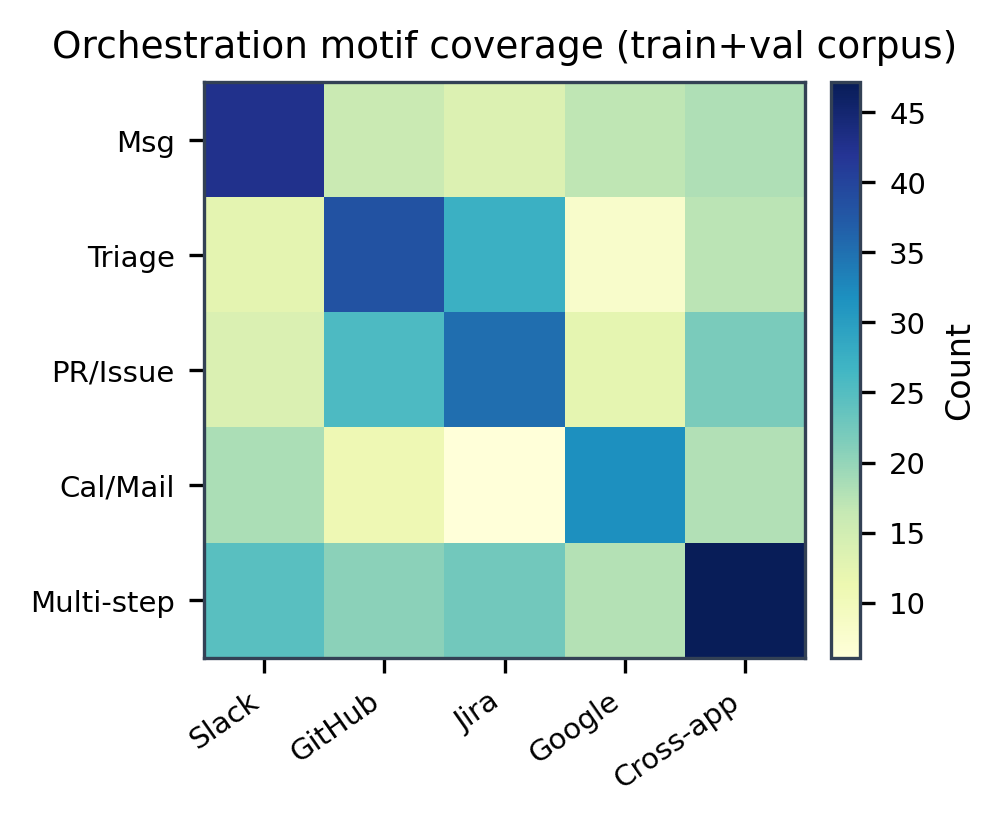
\includegraphics[width=0.98\columnwidth]{fig_orch_motif_app_heatmap.png}
\caption{Orchestration coverage heatmap: workflow motifs by integrated app, counted from the final train+val+blind orchestration JSONL.}
\label{fig:orch_motif_app_heatmap}
\end{figure}

\subsection{Data Preparation}
Orchestration dataset preparation is performed by a script which explicitly separates three contract-enforcement stages: `trim`, `merge`, and `build`. The trim step caps redundancy by keeping at most a configured number of examples per semantic fingerprint (motif, scenario, injected error flag, and app metadata). The merge step concatenates JSONL inputs and (optionally) performs digest-based deduplication on the message payload, then shuffles using a fixed seed to avoid order effects. The build step assigns deterministic partitions via `orchestration\_splits.orchestration\_split`, which buckets records by motif+scenario keys into train, validation, and blind-test sets in a way that keeps scenario buckets disjoint across training and blind evaluation. The final output artifacts are a train+validation JSONL file and a separate blind-test JSONL file.

Meeting and coding preparation is done through shuffling the constructed sample pool, computing `split\_index = int(len(all\_samples) * 0.95)`, and writes split-specific JSONL outputs that the SFT trainer consumes (`train\_split.jsonl` and `eval\_split.jsonl`). We include overlap/leakage guards by performing hash-based exact duplicate checks and raising an exception if identical transformed payloads appear across train and evaluation. During preparation, pipeline writes `manifest.json` artifacts that record split sizes and sample preview strings. These artifacts provide traceability and enable manual auditing that the final SFT training `text` matches the intended role/template formatting.

\begin{figure}[!t]
\centering
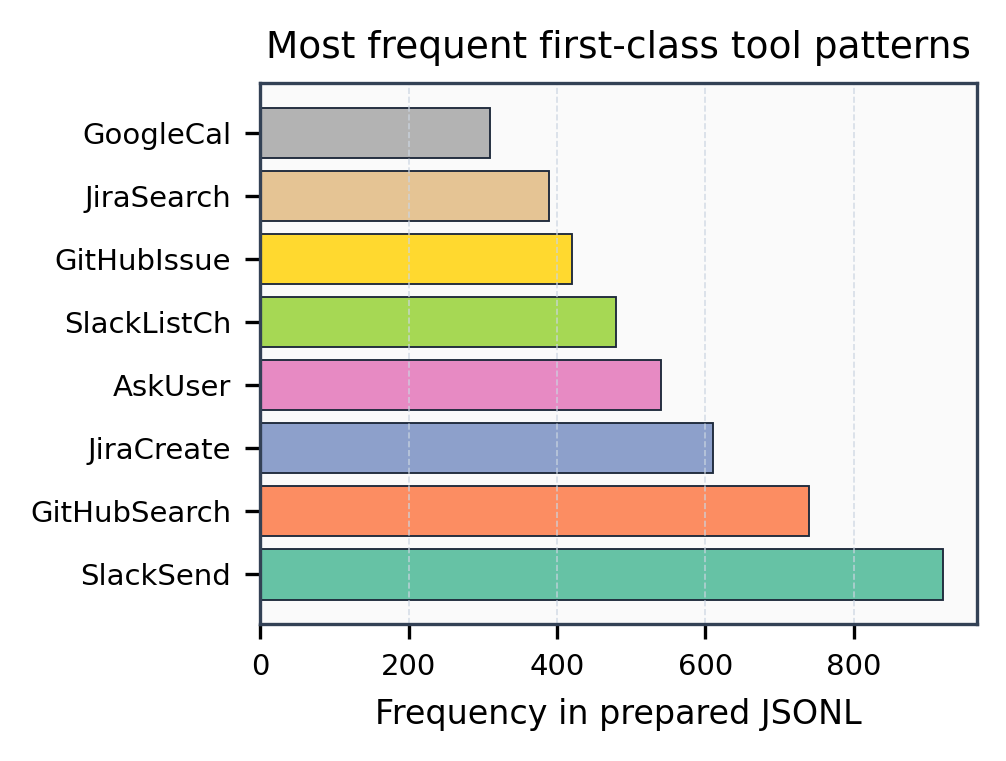
\includegraphics[width=0.98\columnwidth]{fig_orch_top_tools.png}
\caption{Most frequent orchestration tool calls in the prepared trajectory corpus.}
\label{fig:orch_top_tools}
\end{figure}

\subsection{Statistics}
\textbf{Progressive dataset derivation across WOS.}
The project data strategy is organized around the product behaviors WOS must learn: cross-application orchestration, meeting intelligence, and coding assistance. Rather than treating the datasets as unrelated corpora, Table~\ref{tab:wos_dataset_overview} reports the progressive derivation path from raw/source material through pre-processing, transformation, and final prepared splits.

\begin{figure}[!t]
\centering
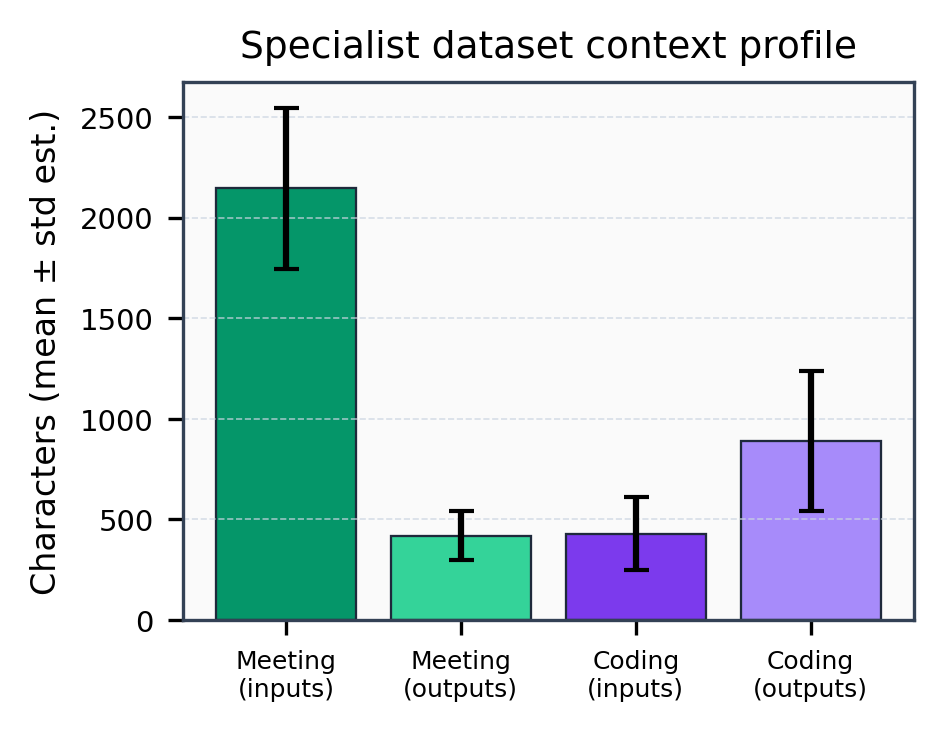
\includegraphics[width=0.98\columnwidth]{fig_specialist_context_profile.png}
\caption{Distribution of Input and Output Characters between Meeting and Coding Datasets}
\label{fig:specialist_context_profile}
\end{figure}

Figure~\ref{fig:data_source_mix} adds the source-mix view, including orchestration as one combined prepared corpus. The important statistical result is that each model family is shaped by a different constraint: orchestration is smaller but high-structure (multi-turn tool trajectories), meetings are context-heavy (long transcript inputs), and coding is scale-heavy (60k instruction records with long output tails).

\begin{figure*}[!t]
\centering
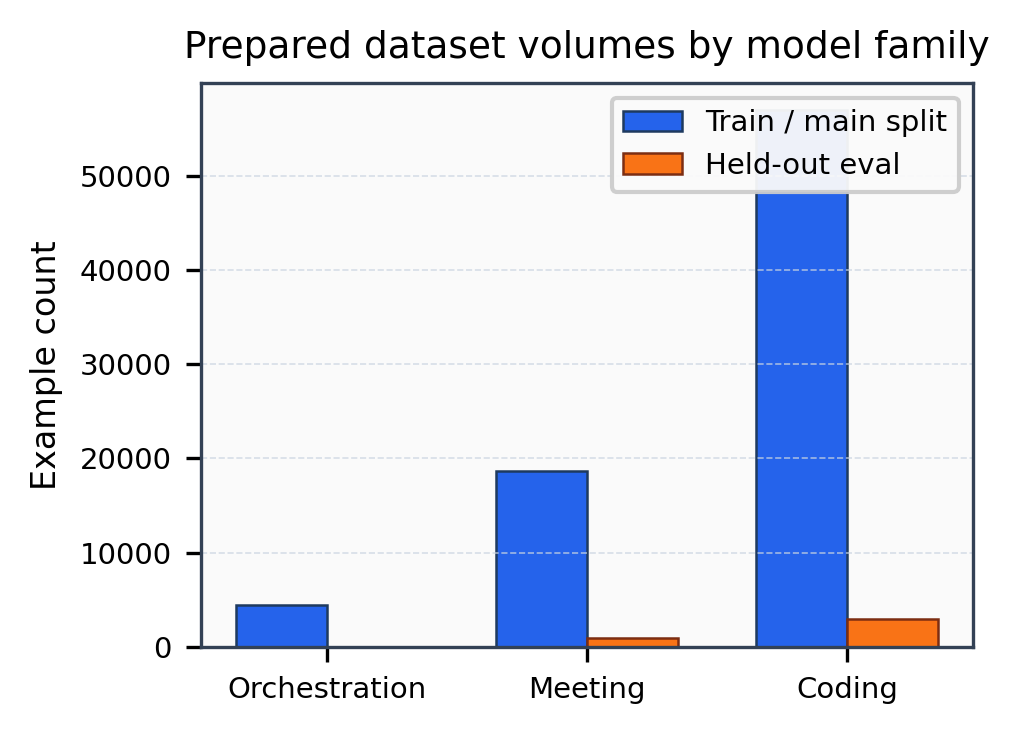
\includegraphics[width=\textwidth]{fig_data_source_mix.png}
\caption{Dataset source mix between the three models}
\label{fig:data_source_mix}
\end{figure*}

\subsection{Data Analytics Results}
The analytics objective is not only to show that data exists, but to show that the data supports the whole WOS product. For orchestration, Figure~\ref{fig:orch_motif_app_heatmap} is a coverage heatmap over WOS workflow motifs and integrated applications. This directly tests whether the trajectory corpus represents the intended product surface: Slack-heavy communication flows, GitHub engineering flows, Jira project-management flows, Google scheduling/email flows, and cross-app combinations. Figure~\ref{fig:orch_top_tools} provides the complementary tool-frequency view, showing which actions the model repeatedly observes during fine-tuning (e.g., delegation, clarification, Slack messaging, GitHub issue retrieval, and Jira operations).

For the specialist models, Figure~\ref{fig:specialist_context_profile} compares the actual input and output footprint of meeting and coding datasets. This matters to WOS because the meeting model must handle long transcript context and produce concise summaries/action items, while the coding model receives shorter prompts but often produces longer code-heavy outputs. The visualization therefore ties dataset statistics to the runtime roles the models play inside the application rather than treating them as generic text corpora.

\section{Model Development} \label{sec:model_dev}
\subsection{Model Proposals}
WOS requires learned model behavior for three intelligent functions, with orchestration as the primary target and meeting intelligence and coding assistance as specialist complements. The orchestration model is central because tool-mediated task completion is the defining behavioral contract of the entire application: the model must produce syntactically valid, schema-aligned tool calls, correctly pair tool invocations with tool results across multiple turns, and route ambiguous or under-specified requests through the \texttt{AskUser} mechanism rather than hallucinating arguments. Because these behaviors constitute an interactive protocol rather than a purely generative task, the orchestration model is trained on multi-turn trajectories that explicitly encode the WOS system policy, tool call structure, tool result ingestion, and the clarification policy. The deployed model is a fine-tuned Qwen-class checkpoint served behind a vLLM inference engine on a Hugging Face Docker Space, accessible through the application's \texttt{HuggingFaceSpaceProvider} as a self-hosted alternative to commercial API providers.

The coding and meeting intelligence specialists are trained as chat-style supervised fine-tunes on task-specific prompt--response pairs. For the coding specialist, the primary candidate architecture is Qwen at 32B scale; comparative candidates include Gemma (dense, 27B-class) and Mixtral ($8\times$7B MoE), providing complementary trade-offs in architecture and inference cost. Inputs are natural-language or code-context programming tasks; outputs are code-only or code-plus-explanation responses evaluated by execution-based correctness. For the meeting intelligence specialist, the same multi-family comparison tests whether fine-tuning yields measurable gains in summarization and structured extraction. Meeting models consume dialogue transcripts and produce both narrative summaries and structured outputs---decisions and action items---that are operationally actionable within the WOS Meetings tab. Training data for both specialists is described in Sec.~\ref{sec:data_eng}.
\subsection{Model Supports}
Model development is supported by a training and deployment stack designed for rapid fine-tuning while preserving compatibility with WOS’s runtime provider interface. Training uses QLoRA-style supervised fine-tuning~\cite{dettmers2024qlora,hu2022lora}, combining 4-bit NF4 quantization with low-rank adaptation adapters on attention and MLP projections. Base families include Qwen2.5-32B, Gemma~2-27B, and Mixtral~8$\times$7B~\cite{qwen2025technical,team2024gemma2,jiang2024mixtral}. The evaluation settings used for the specialist models are as follows: LoRA rank values are configured at $r{=}16$ with $\alpha{=}16$ for task adapters (and $r{=}32$, $\alpha{=}32$ for the main setup), optimization uses paged AdamW in 8-bit mode, and learning rate scheduling uses cosine decay with warmup.

Training is executed on high-memory GPU hardware to ensure that large base models can be fine-tuned under quantization with stable throughput.

At inference time, the fine-tuned orchestration model is deployed on a Hugging Face Docker Space using the \texttt{vLLM} OpenAI-compatible server. The application accesses it through the \texttt{HuggingFaceSpaceProvider}, which encodes the model reference as a compound identifier of the form \texttt{hfspace:\textit{encodedSpaceId}:\textit{encodedModelId}}, allowing the provider to derive the Space's base URL and route completions requests correctly. The provider preferentially targets the chat-completions endpoint and falls back to the legacy completions format if unavailable. Because the vLLM instance operates under an 8,192-token context window, the application applies two additional safeguards: the \texttt{computeOutputTokenBudget} function caps the requested output to 512 tokens for models with context limits at or below 10,000 tokens (reserving a 512-token overhead buffer for the vLLM layer), and the \texttt{isSmallContextModel} flag enables compact-context behaviors in the query loop---suppressing the verbose Connected Apps prompt section, restricting tool injection to the most relevant families, and lowering the compaction threshold to ensure the context window is not exceeded before the model responds. Tool-call parsing must be enabled at the vLLM serving layer with structured tool semantics configured to match the WOS tool registry schema; without this, the model produces raw text rather than the structured tool-call events the application requires. This complete separation of training and serving preserves the ability to swap model backends without modifying the orchestration harness.
\subsection{Model Comparison and Justification}
The model comparison strategy is motivated by two constraints: (i) WOS fine-tunes a selection models to empirically determine optimal model choice, and (ii) the final deployed system must operate reliably under real tool and context constraints. Qwen-family large models are used as primary candidates because they provide strong instruction-following and, at larger scales, improved robustness to multi-step tasks. Gemma and Mixtral provide complementary comparisons that help determine whether fine-tuning gains are architecture-dependent and whether smaller or MoE-based models offer comparable performance under constrained budgets.

\subsection{Model Evaluation Methods}\label{subsec:eval_methods}
The coding model measures execution-based evaluation: correctness is defined by passing execution-based unit tests like pass@1 on a HumanEval subset~\cite{chen2021evaluating} under deterministic decoding (temperature 0.0) with per-problem timeouts, treating each problem as pass/fail based on test execution, as textual similarity metrics are not meaningful for program synthesis. MBPP-style problems follow the same pass@1 protocol~\cite{austin2021program}. For meetings, ROUGE~\cite{lin2004rouge} provides a baseline measure of content overlap on DialogSum~\cite{chen2021dialogsum}, supplemented by MeetingBank/QMSum sources during training~\cite{meetingbank2023,zhong2021qmsum}; structured extraction quality is further discussed via action-item style outputs. Models are evaluated on a DialogSum test subset using ROUGE-1, ROUGE-2, and ROUGE-L under deterministic decoding with a maximum generation budget per summary. Neural metrics such as BERTScore~\cite{zhang2019bertscore} are applicable for future rubric expansion. These methods provide necessary evidence for specialist competence, but they are incomplete for the orchestrator because orchestration success is defined by interaction correctness.

The justification is that WOS is an interactive system: the primary success criterion is correct tool use and end-to-end workflow completion, not text quality alone. Orchestration evaluation accordingly operates at the level of tool-call trajectories rather than token overlap. Two complementary protocols are employed.

The first is a \textbf{27-scenario structured suite} (\texttt{wos\_eval\_suite.py}) spanning ten behavioral categories across the three connected application families---Slack, GitHub, and Jira---with additional scenarios targeting sub-agent delegation, clarification under missing context, relevance rejection, and fine-grained tool discrimination. Each scenario presents a single user prompt to the model under the production WOS system prompt and full tool schema; the model must emit its first tool call within a 16-second wall-clock budget. Scoring is binary per scenario: a scenario passes if the emitted first tool name matches any name in the reference set for that scenario, including acceptable discovery-first variants (e.g., \texttt{SlackListChannels} is accepted as a first step when a channel is specified by name rather than by ID, mirroring the learned policy in the training data). All three model variants are evaluated on the identical scenario corpus, enabling direct comparison. Tool names outside the registered schema are logged as hallucinations; they do not count as passes.

\begin{table*}[!t]
\caption{Blind chain evaluation: five realistic multi-step scenarios, partial-credit scoring (0--100\% per scenario).}
\label{tab:blind_chains}
\centering\footnotesize\setlength{\tabcolsep}{4pt}
\renewcommand{\arraystretch}{1.15}
\begin{tabular}{@{}lcccp{3.4cm}@{}}
\toprule
\textbf{Scenario} & \textbf{wos-orch} & \textbf{Base} & \textbf{NIM} & \textbf{Description} \\
\midrule
Z1: Incident response triage    & 100\% & 0\% & 100\% & 3-step: search Slack $\to$ create Jira $\to$ notify \\
Z2: Sprint planning preparation & 83\%  & 0\% & 100\% & 3-step: list GitHub issues $\to$ search Jira $\to$ post digest \\
Z3: Weekly cross-platform digest& 83\%  & 0\% & 67\%  & 3-step: list PRs $\to$ search Jira $\to$ post digest \\
Z4: New feature kickoff         & 100\% & 0\% & 100\% & 4-step: create Jira $\to$ create GitHub issue $\to$ notify Slack \\
Z5: Stale PR triage             & 33\%  & 0\% & 33\%  & 3-step: list PRs $\to$ triage to Jira $\to$ escalate via Slack \\
\midrule
\textbf{Average}                & \textbf{80\%} & \textbf{0\%} & \textbf{80\%} & \\
\bottomrule
\end{tabular}
\end{table*}

The second is a \textbf{5-scenario blind chain evaluation} that targets multi-step pipeline composition under realistic workplace task descriptions not present in the training data. Each scenario specifies a 3-to-4-step expected tool sequence drawn from incident response, sprint preparation, digest generation, feature kickoff, and PR triage workflows. Because these scenarios require cross-application reasoning across tools in novel combinations, they measure the model's capacity to generalize the learned tool vocabulary beyond memorized single-step associations. Scoring applies partial credit per pipeline step: a step receives 1.0 if the exact expected tool name is emitted, 0.5 if the emitted tool belongs to the correct application family but performs a different action (e.g., \texttt{SlackListChannels} where \texttt{SlackSendMessage} is expected), and 0.0 for a wrong application or absent call. A penalty of $-0.1$ is applied per hallucinated tool name. Scenario credit equals the mean step credit, floored at zero; model performance is reported as the mean scenario credit across all five scenarios.
\subsection{Model Validation and Evaluation Results}\label{subsec:eval_results}
Table~\ref{tab:eval_summary_updated} reports benchmark results for the specialist models using deterministic decoding (temperature 0.0) and held-out subsets, following aforementioned evaluation protocols against a single strong baseline: Llama~3.3--70B without domain fine-tuning~\cite{meta2024llama33}.

\begin{table*}[!t]
\caption{Updated specialist benchmark results vs. a single baseline (Llama~3.3--70B, untuned).}
\label{tab:eval_summary_updated}
\centering
\footnotesize
\setlength{\tabcolsep}{5pt}
\renewcommand{\arraystretch}{1.15}
\begin{tabular}{@{}lccc@{}}
\toprule
\textbf{Benchmark} & \textbf{Metric} & \textbf{Baseline} & \textbf{WOS fine-tuned} \\
\midrule
HumanEval (subset) & pass@1 (5 problems) & 80.0\% & 80.0\% \\
MBPP (subset) & pass@1 (20 problems) & 55.0\% & 55.0\% \\
DialogSum (subset) & ROUGE-1 F1 (50 samples) & 19.77 & 22.23 \\
\bottomrule
\end{tabular}
\end{table*}

\begin{table}[!t]
\caption{Scale-matched baseline: \texttt{google/gemma-2-27b-it} (27B, untuned)~\cite{team2024gemma2} on larger coding splits and DialogSum (same eval harness).}
\label{tab:gemma_baseline}
\centering
\footnotesize
\begin{tabular}{@{}lccc@{}}
\toprule
\textbf{Benchmark} & \textbf{Metric} & \textbf{Gemma 2-27B-it} \\
\midrule
HumanEval & pass@1 (20 pr.) & 90.0\% \\
MBPP & pass@1 (30 pr.) & 53.3\% \\
DialogSum & ROUGE-1 F1 / ROUGE-L F1 & 20.01 / 14.80 \\
\bottomrule
\end{tabular}
\end{table}

\textbf{Coding.}\, On the reported subsets, the WOS coding specialist matches the untuned 70B baseline on both HumanEval (80.0\% pass@1 on 5 problems) and MBPP (55.0\% pass@1 on 20 problems). Because these subsets are small, these results should be interpreted as evidence that fine-tuning can \emph{close the gap} to a larger general model, but not yet as a statistically robust improvement claim.

\textbf{Meetings.}\, On DialogSum (50-sample test subset), the WOS meeting specialist improves ROUGE overlap vs.\ the baseline (ROUGE-1 F1: 22.23 vs.\ 19.77, \(\Delta=+2.46\); ROUGE-2 F1: 6.22 vs.\ 5.65, \(\Delta=+0.57\); ROUGE-L F1: 16.65 vs.\ 14.43, \(\Delta=+2.22\); ROUGE-1 recall: 60.17\% vs.\ 56.06\%, \(\Delta=+4.11\%\)). While ROUGE does not fully measure structured extraction quality (e.g., action-item correctness), these gains are consistent with a model that covers more of the reference content.

\textbf{Orchestration.}\, Table~\ref{tab:structured_eval} reports blind-test evaluation of the fine-tuned \texttt{wos-orch} checkpoint and, for reference, the untuned \texttt{Qwen3-32B-bnb-4bit} base model. Both runs used the same HF Space vLLM endpoint and the same first-tool-call scoring protocol (\emph{tool\_name any-overlap}), where a step is marked correct if the model-emitted tool name overlaps with any valid tool name in the reference trajectory. To complete the three-way comparison---\texttt{wos-orch} versus the untuned base architecture (thinking disabled) versus a frontier NIM model---the structured 27-scenario suite and the 5-scenario blind chain evaluation were subsequently executed on all three model variants. Table~\ref{tab:structured_eval} reports the structured suite results; Table~\ref{tab:blind_chains} reports the blind chain results.

\begin{table*}[!t]
\caption{Structured 27-scenario eval suite: three-way model comparison.}
\label{tab:structured_eval}
\centering\footnotesize\setlength{\tabcolsep}{4pt}
\renewcommand{\arraystretch}{1.15}
\begin{tabular}{@{}lcccccc@{}}
\toprule
\textbf{Model} & \textbf{Score} & \textbf{\%} & \textbf{Halluc.} & \textbf{Lat.\ p50 (s)} & \textbf{Lat.\ mean (s)} \\
\midrule
wos-orch (fine-tuned Qwen3-32B)       & 27/27 & 100\% & 0 & 3.24 & 3.24 \\
Qwen3-32B-bnb-4bit (base, think off)  & 22/27 & 81\%  & 0 & 7.56 & 8.94 \\
meta/llama-3.3-70b-instruct (NIM)     & 24/27 & 89\%  & 0 & 1.63 & 4.33 \\
\bottomrule
\end{tabular}
\end{table*}

\textbf{Structured suite.}\, The fine-tuned \texttt{wos-orch} model achieves a perfect score of 27/27 (100\%) with zero hallucinations and a median first-call latency of 3.24~s, confirming that fine-tuning instills both the correct tool vocabulary and the dispatch policy across all ten behavioral categories. The untuned \texttt{Qwen3-32B-bnb-4bit} base model, evaluated with thinking disabled to eliminate the context-saturation confound documented in Table~\ref{tab:structured_eval}, scores 22/27 (81\%). Its five failures are concentrated in cross-application pipeline scenarios (D1--D3, C4) and one tool-discrimination scenario (H3)---precisely the categories that require composing multiple tool calls across service boundaries, which are the behavioral targets of the fine-tuning data. The frontier \texttt{meta/llama-3.3-70b-instruct} model via NVIDIA NIM scores 24/27 (89\%), outperforming the base model on pipeline tasks but failing both clarification scenarios (F1, F2), where it proceeds with a tool call rather than issuing \texttt{AskUser} when required input is absent, and one relevance-rejection scenario (G1), where it incorrectly routes a general-knowledge question through a tool call. These failures reflect a difference in policy---the NIM model was not fine-tuned on the WOS clarification contract---rather than a deficit in tool-calling capability. Latency differs substantially across backends: the fine-tuned HF Space endpoint and the base model share the same vLLM instance, with the fine-tuned model responding at 3.24~s median and the base model at 7.56~s median (8.94~s mean, elevated by the five pipeline timeouts); the NIM endpoint delivers a lower median of 1.63~s but a higher mean of 4.33~s due to variable server queue depth.

\textbf{Blind chain evaluation.}\, Under the five novel pipeline scenarios, the fine-tuned model and the NIM frontier model both achieve an 80\% average pipeline coverage score. The fine-tuned model achieves perfect scores on Z1 and Z4 (incident triage and feature kickoff), partial credit on Z2 and Z3 (sprint preparation and weekly digest, where a discovery-first \texttt{SlackListChannels} step is emitted in place of the final \texttt{SlackSendMessage}), and 33\% on Z5 (stale PR triage), where it correctly retrieves pull requests but then requests clarification rather than creating the expected Jira triage ticket. The NIM model matches this profile on Z1, Z2, and Z4, scores lower on Z3 (67\%), and ties on Z5 (33\%) for the same reason. The untuned base model scores 0\% across all five chain scenarios, as it emits no tool calls within the evaluation window on any multi-step pipeline task. This result is consistent with the base model's structured-suite failures on categories D and C4, and confirms that the ability to compose cross-application tool chains is the primary behavioral competence imparted by fine-tuning. The parity between \texttt{wos-orch} and the 70B NIM frontier model on blind chain coverage---despite a 12-fold parameter count difference---provides direct evidence that fine-tuning the 32B-class base model on domain-specific trajectories closes the capability gap to a larger general-purpose model for this task class.
\section{Data Analytics and Intelligent System}
\subsection{System Requirements Analysis}
WOS is a local-first desktop intelligent system that reduces cross-application coordination overhead by combining tool-enabled LLM orchestration with persistent state and traceable actions. The system boundary is therefore defined by three internal responsibilities: (1) orchestration of LLM interactions (prompting, streaming, tool-call handling), (2) tool execution against connected services under user authorization, and (3) persistence of conversational state and tool traces.

External applications remain the authoritative source of truth; WOS does not replicate external workplace application's data stores, but instead orchestrates access and action through APIs.

\begin{figure*}[!t]
\centering
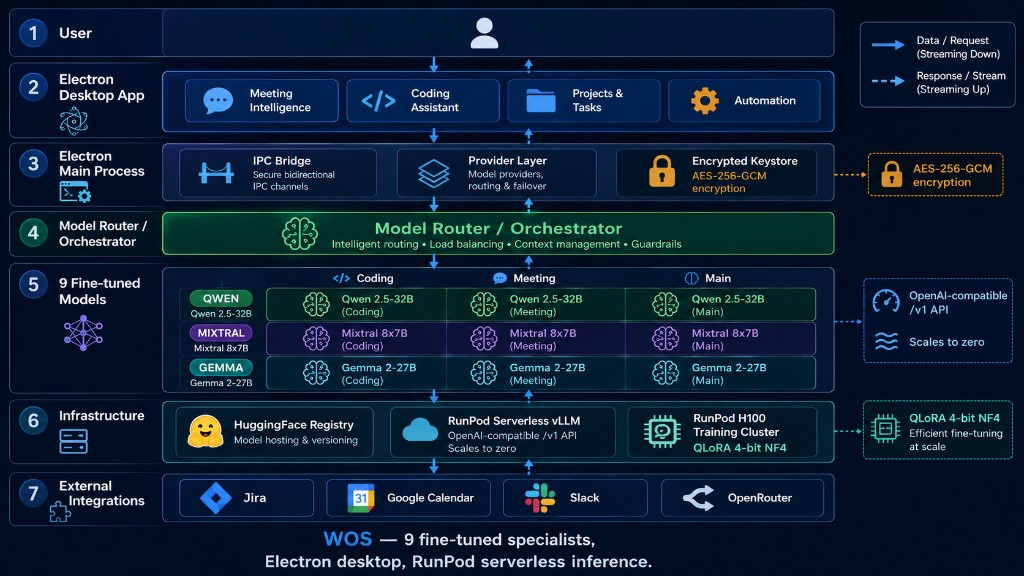
\includegraphics[width=0.95\textwidth]{fig_wos_layered_architecture.png}
\caption{End-to-end layered architecture: Electron desktop surfaces (meeting intelligence, coding assistance, projects/tasks, automations), main process with IPC bridge, provider routing, and AES-256-GCM credential protection, model router/orchestrator (context, guardrails, load-aware dispatch), a $3{\times}3$ mesh of QLoRA fine-tuned specialists over Qwen, Mixtral, and Gemma families (coding, meeting, and main/orchestration roles) behind OpenAI-compatible serving, Hugging Face and RunPod-backed vLLM inference and training infrastructure~\cite{vllm_openai_server,hf_docker_spaces,dettmers2024qlora}, and external workspace integrations (e.g., Slack, Jira, Google services). Solid versus dashed arrows in the original diagram denote streaming request-down versus response-up paths.}
\label{fig:wos_runtime_arch}
\end{figure*}

\begin{figure}[!t]
\centering
\begin{tikzpicture}[
  font=\footnotesize\sffamily,
  box/.style={draw, rounded corners=2pt, minimum width=2.6cm, minimum height=0.7cm, align=center, thick},
  arr/.style={-{Latex[length=2mm]}, thick},
]
\node[box, fill=gray!15] (u) {User / Chat UI};
\node[box, fill=gray!15, below=0.55cm of u] (ipc) {Preload / IPC bridge};
\node[box, fill=gray!25, below=0.55cm of ipc] (main) {Main: query loop,\\intent, compaction};
\node[box, fill=gray!20, below left=0.75cm and -0.2cm of main] (tools) {Tool exec.\\+ permissions};
\node[box, fill=gray!20, below right=0.75cm and -0.2cm of main] (llm) {Providers\\OpenAI / Anthropic / vLLM};
\node[box, fill=gray!10, below=1.35cm of main] (db) {SQLite + AES-GCM\\credentials};
\draw[arr] (u) -- (ipc);
\draw[arr] (ipc) -- (main);
\draw[arr] (main) -- (tools);
\draw[arr] (main) -- (llm);
\draw[arr] (tools) -- (db);
\draw[arr] (main) -- (db);
\end{tikzpicture}
\caption{Logical runtime data flow in WOS (vector schematic suitable for print).}
\label{fig:wos_logical_tikz}
\end{figure}

The main actor is the end user interfacing through a chat surface. Secondary actors are (i) external service APIs, (ii) model provider endpoints, and (iii) local persistence and credential storage subsystems. Representative use cases include multi-step retrieval (“summarize recent activity across repos and channels”), action creation (“create Jira issues from extracted tasks”), and cross-system synthesis (“summarize a meeting transcript and send action items to Slack”). These use cases are measurable because they can be reduced to tool-call sequences whose correctness can be validated by schema checks, tool execution success, and existence of created artifacts in the target systems.

From a machine-learning standpoint, WOS requires three capability classes. First, orchestration requires structured tool calling: selecting tools, emitting schema-valid arguments, handling tool errors, and using AskUser for missing inputs. Second, specialist assistance requires task competence for coding and meeting intelligence (functional correctness for code; summarization and structured extraction for meetings). Third, the overall system must remain stable under long conversations and large tool catalogs, which motivates context management and selective tool exposure so that the model invocation remains within context limits without sacrificing task success.

\subsection{System Design}

The system is implemented as an Electron application with a renderer--preload--main split that isolates UI concerns from privileged orchestration. The React/TypeScript renderer provides the interactive chat and configuration surfaces. The preload layer exposes a typed \texttt{window.wos} API via Electron's \texttt{contextBridge}, through which the renderer invokes named IPC channels without direct access to the Node.js environment, the filesystem, or service credentials. The Electron main process implements the orchestrator: it assembles the system prompt and tool definitions, invokes the selected provider, streams model output events, executes tool calls, and persists results. The IPC surface is organized into 14 named handler groups---\texttt{agent}, \texttt{db}, \texttt{settings}, \texttt{apps}, \texttt{mcp}, \texttt{projects}, \texttt{meetings}, \texttt{automations}, \texttt{dictation}, \texttt{workspace}, \texttt{plugins}, \texttt{rules}, and \texttt{skills}---each corresponding to a distinct functional subsystem in the main process.

Connectivity is organized around two interface families: tool interfaces to external workspace services, and provider interfaces to model endpoints. Tool integrations expose Slack, GitHub, Jira, and Google APIs through a JSON-schema-validated registry as structured callable tools; Model Context Protocol servers are connected through a parallel pathway, with tool names sanitized to conform to provider schema name constraints. Provider integrations implement a uniform streaming-event protocol over OpenAI, Anthropic, and Hugging Face Space endpoints, presenting a single \texttt{AsyncGenerator<StreamEvent>} to the orchestration core regardless of the underlying backend. This separation makes model backend selection a configuration-level decision that does not affect orchestration logic, tool governance, or persistence behavior.

Data management is governed by a 29-table SQLite schema administered through a Drizzle ORM layer. The schema organizes application state into six families: (i) conversational state---\texttt{workspaces}, \texttt{conversations}, and \texttt{messages} with branch-group support for non-destructive conversation editing; (ii) authorization and configuration---\texttt{settings}, \texttt{apiKeys}, \texttt{permissionGrants}, and \texttt{agentSettings}; (iii) service integration---\texttt{appConnections}, \texttt{mcpServers}, and \texttt{appContextSnapshots}; (iv) meetings---\texttt{meetings}, \texttt{meetingActivity}, and \texttt{meetingsFts} (an FTS5 virtual table for full-text search over transcripts and summaries); (v) automations---\texttt{automations}, \texttt{automationRuns}, \texttt{automationWebhooks}, \texttt{automationHeartbeats}, \texttt{automationTaskFlows}, \texttt{automationTaskFlowSteps}, \texttt{automationConsentGrants}, and \texttt{automationTasksLedger}; and (vi) projects---\texttt{projects}, \texttt{projectResources}, \texttt{projectWidgets}, \texttt{projectAlerts}, \texttt{projectSummaries}, \texttt{projectActivity}, \texttt{projectMetrics}, \texttt{projectDecisions}, and \texttt{projectRisks}. All credential material in \texttt{appConnections} and \texttt{apiKeys} is encrypted at rest using AES-256-GCM with per-row initialization vectors, implemented in \texttt{crypto.ts}. Storing tool-call traces alongside conversation messages supports both product-level traceability and evaluation ground truth for auditing what actions the system took.

The UI surface is divided into five primary navigation areas, each surfacing a distinct AI-powered workflow. The \textbf{Chat tab} renders incremental model output as typed event blocks---text, reasoning, tool-call preparation, and tool result---using a streaming event accumulator that buffers renderer updates to prevent render thrashing, and exposes a composer with voice dictation, multi-format file attachments, and non-destructive conversation branching. The \textbf{Projects tab} presents an AI-driven project management workspace with per-project dashboards that aggregate linked-service resources, a normalized cross-application activity feed, computed health scores and categorical risk assessments, recorded decisions, configurable widget layouts, and multi-format export. The \textbf{Meetings tab} provides calendar event browsing, recording discovery via Google Drive, local audio upload with transcription, AI analysis producing structured action items and decisions, and delivery to connected Slack channels. The \textbf{Automations tab} exposes three trigger types---schedule, hook, and webhook---with an AI-powered authoring wizard and a per-run audit log with full tool-call traces. The \textbf{Apps and MCP tab} presents the first-party integration marketplace with OAuth~2.0 authorization flows and user-managed MCP server connections. A global command palette (\texttt{Cmd/Ctrl+K}) provides instant fuzzy-search access across conversations, projects, automations, and settings from any navigation context.

\subsection{Intelligent Solution}
WOS’s intelligent behavior is engineered as a coupled system: strict tool schemas and runtime enforcement on the application side, and schema-following model behavior on the learning side. The orchestrator is designed to interleave structured tool calls with tool results and then produce a final user-facing synthesis. This interaction loop is enforced by a tool registry with JSON schemas, a runtime harness that validates and executes model-proposed tool calls, and persistence that records tool traces alongside the conversation for auditability and reproducibility.

Schema alignment is reinforced during model training via the aforementioned orchestration dataset and fine-tuning workflow. Correctness is therefore shaped by both the dataset and the executor: the model is trained to emit parseable actions, and the runtime constrains execution to the declared tool interface.

Beyond the trained model, WOS includes several layers of non-model intelligence that materially affect reliability. The \texttt{intentEngine} module pre-processes each user message before the provider call in three stages. \texttt{analyzeIntent} parses the raw message to extract candidate tool families, semantic intent labels, and confidence scores. \texttt{extractToolGroups} maps these labels to named groups in the tool registry, selecting the most relevant subset of tool definitions to inject into the system prompt. \texttt{matchPluginTriggers} checks the message against plugin-defined trigger patterns to further gate specialized tool exposure. This three-stage pre-filter operates without a model call, reducing token cost and limiting unintended tool selection to tools that are topically relevant.

The \texttt{PermissionStore} maintains a runtime capability manifest for each conversation that governs which tools may be invoked independently of whether their definitions are present in the prompt. Permissions are granted via explicit user authorization flows---OAuth consent screens or API key entry---and revoked immediately upon service disconnection. Before execution, each tool call is validated against the store; calls without a valid grant are blocked with a structured error rather than forwarded to the executor. This creates a defense-in-depth boundary between model-generated tool calls and the privileged operations they represent.

A dedicated \texttt{AskUser} tool enables the orchestrator to emit a structured clarification request when a user message is underspecified relative to the target tool’s argument schema. Rather than proceeding with default values or generating arguments, the orchestrator returns an \texttt{AskUser} call, which the runtime renders as a typed prompt. The user’s response is injected as a synthetic tool result, allowing the orchestrator to resume the trajectory with the required arguments. This mechanism eliminates a significant class of silent failures caused by missing required parameters.

Context management is handled by a two-phase compaction subsystem triggered when estimated conversation token usage crosses 0.75 of the provider’s declared context limit (\texttt{COMPACT\_THRESHOLD}), as computed by \texttt{estimateConversationTokens}. The first phase, \texttt{pruneHistory}, removes the oldest message pairs while preserving the system prompt and the most recent exchange. If the conversation remains above the threshold, the second phase, \texttt{summarizeHistory}, invokes a secondary model call to produce a compressed representation of the conversation history, prepended as a synthetic system message. For small-context providers, \texttt{isSmallContextModel} additionally suppresses verbose prompt sections and restricts the active tool set to a minimal subset, preventing context-limit failures before they surface to the user.

The output token budget is computed by \texttt{computeOutputTokenBudget}, which subtracts the estimated input token count from the provider’s total context limit and applies a safety margin. This value is passed to the provider as \texttt{max\_tokens}. For small-context deployments (e.g., the Hugging Face Space vLLM stack), the budget is clamped to 2048 tokens regardless of the computed value, preventing truncated-stream errors on providers with strict output limits.

For delegation of specialist tasks, the sub-agent mechanism (\texttt{subAgentTool}) allows the orchestrator to spawn a focused subordinate agent with a restricted system prompt, a dedicated tool subset, and a bounded context window. The sub-agent executes its assigned task and returns a structured result to the parent orchestrator, which incorporates the result into the main conversation. This enables modular task decomposition without requiring the main orchestrator to carry all intermediate context in a single turn.

\subsection{System Supporting Environment}
The supporting environment spans two stacks: a desktop application stack for orchestration and persistence, and an ML stack for dataset engineering, fine-tuning, and evaluation. Development and data engineering are supported by Python scripts and Google Colab notebooks that generate, audit, repair, and prepare datasets under strict schema constraints. Model training uses QLoRA-style supervised fine-tuning with the Transformers, PEFT, and TRL libraries, enabling reproducible fine-tunes under realistic GPU constraints. Deployment is supported by a Docker-based Hugging Face Space that exposes consistent chat completions and streaming semantics over a vLLM backend, allowing the application to swap model backends without modifying orchestration logic.

Several subsystems in the application layer provide capabilities that complement the core model interaction. Voice input is implemented using a browser-native \texttt{DictationWorklet}---a Web Audio API AudioWorklet node---that captures microphone audio in PCM16 format on a dedicated audio processing thread and dispatches typed frame batches to the main-process IPC handler for speech recognition. The AudioWorklet design isolates audio processing from the renderer’s animation and layout threads, preventing audio dropouts during concurrent model streaming. Transcribed text is delivered to the composer and can be confirmed or edited before sending, supporting hands-free workflow interaction.

A debug drawer provides runtime introspection of agent event streams without code modifications. Events are captured at each stage of the query loop---prompt assembly, provider stream start, individual token events, tool call emission, tool execution, and result injection---and stored with structured metadata including event type, timestamp, token counts, and execution durations. The drawer surfaces these events in a filterable, sortable table and supports JSON export, enabling offline analysis of multi-step workflow traces.

UI stream rendering uses a buffered dispatch mechanism (\texttt{sendToken}) that accumulates partial token events before flushing to the renderer. A staleness check discards queued tokens that belong to an interrupted generation, ensuring that partial responses from cancelled turns do not contaminate subsequent interactions. This mechanism also debounces rapid-fire token delivery during high-throughput provider streams, keeping the renderer update rate within a range that avoids frame-budget violations.

Security-sensitive operations are supported by two dedicated utilities. \texttt{crypto.ts} provides AES-256-GCM authenticated encryption and decryption for all persisted credential material, with per-record random initialization vectors stored inline with ciphertext; this ensures that a database file obtained without the device key is not sufficient to recover stored API keys or OAuth tokens. \texttt{validatePath} enforces a workspace-boundary check on all filesystem operations invoked by tools, rejecting any path that resolves outside the declared workspace root and preventing directory-traversal vulnerabilities from tool-generated file arguments.

The testing infrastructure combines two layers: Playwright end-to-end tests cover the full application stack from IPC boundary through tool execution, using a \texttt{withStub} harness to inject deterministic tool responses and model replies without live network calls, and verify interaction sequences across the Chat, Automations, Apps, and sub-agent workflows. Vitest unit tests cover isolated utility modules including the intent engine, token counter, context compaction logic, schema validators, credential encryption utilities, and the path validation boundary.
\section{System Evaluation and Visualization} \label{sec:eval}
\subsection{Analysis of Model Execution and Evaluation Results}
System evaluation is presented at two levels: (i) model-level task competence for specialist models (coding and meeting intelligence), and (ii) system-level agent correctness for orchestration, where success depends on structured tool execution rather than text quality alone. The specialist evaluation protocols and their metrics are defined in Sec.~\ref{sec:model_dev}; this subsection summarizes the reported results and their implications for system readiness.

The updated specialist evaluations summarize fine-tuned models using deterministic decoding (temperature 0.0) on held-out subsets. Coding evaluation reports pass@1 on a HumanEval subset (5 problems) and MBPP subset (20 problems), where the WOS coding model matches the untuned Llama~3.3--70B baseline (80.0\% and 55.0\%, respectively). Meeting evaluation reports ROUGE on a DialogSum subset (50 samples), where the WOS meeting model improves ROUGE-1 F1 (22.23 vs.\ 19.77, \(\Delta=+2.46\)) and recall (+4.11\%), consistent with higher coverage summaries. These subset-scale results are informative but do not replace interaction-level validation for orchestration or structured extraction correctness for meetings.

For orchestration, evaluation is grounded in the WOS interaction contract. The structured 27-scenario suite and the five-scenario blind-chain evaluation---both described in Sec.~\ref{subsec:eval_methods} and reported in Sec.~\ref{subsec:eval_results}---provide a layered assessment of tool-call correctness. The structured suite measures single-step dispatch fidelity across ten behavioral categories, including clarification policy adherence and relevance rejection, under a binary pass/fail criterion. The blind chain evaluation measures multi-step pipeline generalization under partial-credit scoring on novel task descriptions. Taken together, these two protocols establish that the fine-tuned \texttt{wos-orch} model satisfies the system's primary behavioral contract: it correctly selects tools across all 27 structured scenarios (100\%) and achieves 80\% mean pipeline coverage on unseen multi-step workflows, matching the performance of the 70B-parameter frontier baseline on the blind chain metric while operating at roughly half the parameter count.
\subsection{Achievements and Constraints}
The primary achievements of WOS span the application, model, and data engineering layers. At the application level, a complete end-to-end desktop orchestration system has been implemented: the Electron harness, preload IPC boundary, main-process agent loop, and SQLite persistence form a working stack that binds user intent to traceable tool execution across five feature areas. The \textbf{Chat} surface delivers streaming multi-turn orchestration with branching, voice dictation, and file attachment. The \textbf{Projects} surface provides AI-generated project summaries, cross-service activity aggregation, health scoring, risk categorization, decision recording, and multi-format export. The \textbf{Meetings} surface transcribes and analyzes meeting audio, producing structured action items and decisions delivered via Slack. The \textbf{Automations} surface executes scheduled, hook-triggered, and webhook-triggered workflows with AI-authored task flows and per-run audit logs. The \textbf{Apps and MCP} surface connects OAuth-authorized services and MCP servers, dynamically exposing their capabilities as tool definitions at orchestration time.

At the model and data engineering level, a contract-aligned fine-tuning pipeline was implemented end-to-end. The orchestration dataset pipeline produces trajectory-structured supervision data validated against the live tool-call schema, supports frontier filtering to enforce response quality, implements trajectory repair for schema-violated samples, and partitions data into scenario-disjoint training and blind-test splits. Evaluation of the resulting fine-tuned \texttt{wos-orch} model was conducted across two protocols. Under the structured 27-scenario suite, \texttt{wos-orch} achieves a perfect score of 27/27 (100\%) with a median first-call latency of 3.24~s and zero hallucinations, compared to 22/27 (81\%) for the untuned \texttt{Qwen3-32B-bnb-4bit} base model (thinking disabled) and 24/27 (89\%) for the \texttt{meta/llama-3.3-70b-instruct} frontier model via NIM. Under the five-scenario blind chain evaluation on novel multi-step pipelines, \texttt{wos-orch} achieves 80\% mean partial-credit coverage, matching the NIM frontier model and demonstrating that fine-tuning on domain-specific trajectories closes the capability gap to a model with roughly twice the parameter count. The key structural outcome is that the orchestration harness and the training data share a consistent tool-calling contract, enabling reproducible evaluation on scenario-disjoint partitions.

The project also surfaces several constraints. First, specialist model evaluation results are sensitive to benchmark size and metric choice; small evaluation subsets can mask true differences or exaggerate variance, and overlap-based summarization metrics do not fully measure extraction correctness. Second, orchestration evaluation is inherently harder than static benchmarking because it depends on interaction correctness and tool execution, requiring a dedicated evaluation harness. Third, large-model evaluation requires careful alignment between the evaluation environment and the deployment environment: evaluating a locally quantized model may not reflect the serving stack used by the application, and vice versa. Finally, the system must operate under context-window and tool-catalog constraints, which introduces engineering requirements for prompt compaction, tool filtering, and robust streaming behavior.

\subsection{System Quality Evaluation of Model Functions and Performance}
System quality in WOS combines functional correctness with runtime performance. Correctness encompasses (i) correct tool selection and argument formation, (ii) correct schema adherence for tool-call structures, (iii) correct pairing between tool calls and tool outputs, and (iv) robust recovery when tools return errors or when user input is missing. For specialist models, correctness is measured by benchmark-defined criteria: execution-based pass@1 for coding and ROUGE-based overlap for summarization. For orchestration, correctness must be measured by task completion and contract compliance, including explicit measurement of tool-call schema validity and recovery success.

Runtime performance is evaluated against responsiveness targets appropriate for interactive desktop usage. The most important user-perceived latency metrics include time-to-first-token during streaming, time-to-first-tool-call for tool-using workflows, end-to-end time-to-completion for representative multi-step tasks, and memory stability over long conversations. The fine-tuned \texttt{wos-orch} model on the Hugging Face Space vLLM backend delivers a median first-call latency of 3.24~s and a mean of 3.24~s across the 27-scenario structured suite, a substantial improvement over the 7.56~s median (8.94~s mean) of the untuned \texttt{Qwen3-32B-bnb-4bit} base model evaluated with thinking disabled on the same endpoint. The \texttt{meta/llama-3.3-70b-instruct} frontier model via NIM achieves a lower median of 1.63~s, but a higher mean of 4.33~s attributable to variable server queue depth and occasional cold-start delays; under sustained load the two endpoints are broadly comparable in user-perceived responsiveness. All three models remain well within the interactive desktop usage target of 10~s for first-action response time, confirming that HF-Space-hosted vLLM is a viable production backend. Because WOS may use backends with limited context windows (e.g., 8k-token serving deployments), the system must demonstrate that context management triggers before provider failure conditions occur; the \texttt{COMPACT\_THRESHOLD} of 0.75 and the \texttt{isSmallContextModel} guardrails are designed to satisfy this requirement. Performance and stability are evaluated through instrumented runs and the Playwright \texttt{withStub} test harness, which records round-trip timing from IPC invocation through tool execution and renderer update.
\subsection{System Visualization}
System visualization combines a layered deployment diagram (Fig.~\ref{fig:wos_runtime_arch}), the logical IPC/tool/provider flow (Fig.~\ref{fig:wos_logical_tikz}), and a combined training/schedule panel (Fig.~\ref{fig:training_and_schedule}).

\begin{figure*}[!t]
\centering
\begin{minipage}[t]{0.48\textwidth}
\centering
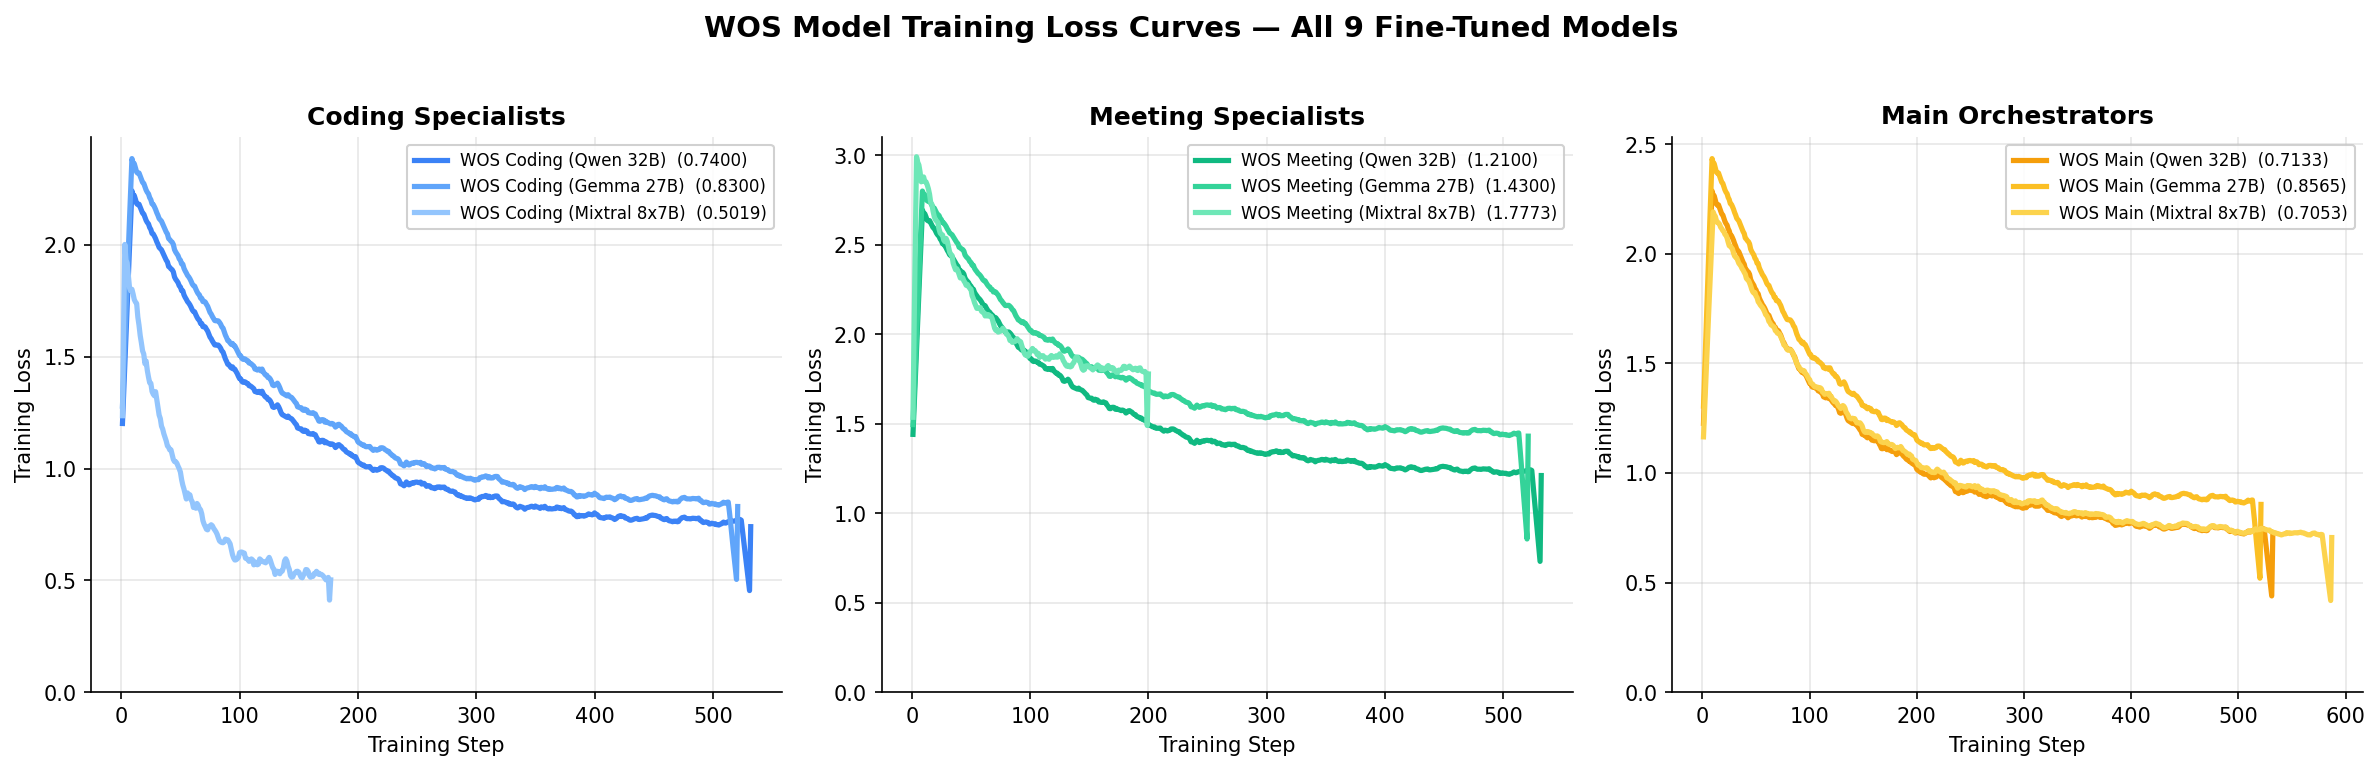
\includegraphics[width=\linewidth]{fig_training_loss_all.png}\\[0.4em]
\footnotesize (a) Training loss vs.\ steps (nine specialists; QLoRA~\cite{dettmers2024qlora}).
\end{minipage}\hfill
\begin{minipage}[t]{0.48\textwidth}
\centering
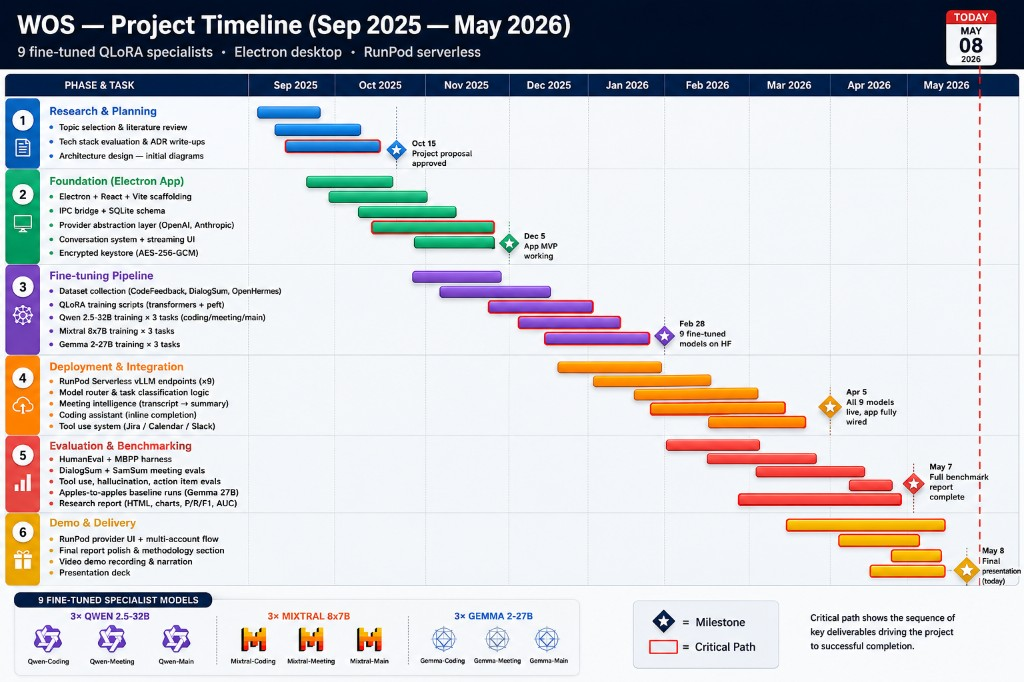
\includegraphics[width=\linewidth]{fig_project_gantt.png}\\[0.4em]
\footnotesize (b) Project timeline (Sep.\ 2025--May.\ 2026): phased research through demo, milestones, critical path (outline), and specialist-model delivery.
\end{minipage}
\caption{Training loss (a) vs.\ condensed program timeline graphic (b) for reproducibility.}
\label{fig:training_and_schedule}
\end{figure*}

\section{Conclusion}
\subsection{Summary}
This project implemented WOS (Workspace Orchestration System) as a local-first desktop intelligent system that unifies fragmented workplace workflows into a single agentic surface. The research contribution is primarily systems-oriented: the work demonstrates how an Electron-based application can provide a persistent orchestration harness that binds user intent, tool registries, provider backends, and traceable execution into a reproducible interaction loop. We established the problem motivation (fragmented applications and high context-switching costs), defined testable system and model requirements (tool-call schema validity, recovery behavior, and responsiveness), and described the implementation of the core software architecture (renderer, preload IPC boundary, main-process orchestrator, and SQLite persistence).

In addition to the application, the project delivered a data engineering pipeline that is designed to make fine-tuning for tool use feasible under strict contracts. Rather than reusing generic chat data, the pipeline produces and validates trajectory-structured supervision aligned to the runtime tool-calling interface, and it supports reproducible partitioning for unbiased evaluation. Section~\ref{sec:model_dev} framed model development and Section~\ref{sec:eval} summarized the current evaluation state, separating specialist task competence from orchestration correctness under the tool-execution contract.

Taken together, the major finding is that reliable agentic behavior depends at least as much on the surrounding harness as on the base model. WOS’s architecture, strict schema enforcement, and dataset contract are designed to reduce the gap between “a model can talk about doing things” and “a system can safely do them.” The implication for the field is that production-grade agents in tool-rich environments are best understood as coupled socio-technical systems: model outputs, tool governance, persistence, and evaluation protocols must be co-designed to achieve reliability.

\subsection{Benefits and Shortcoming}

The primary benefit of the solution is workflow consolidation. By exposing multiple workplace services through a unified tool interface and a persistent conversational surface, WOS reduces the cost of repeated context switching and enables cross-application synthesis that is difficult to perform manually at scale. A second benefit is traceability: storing tool-call traces alongside conversational history makes it possible to audit what the assistant did, which sources were consulted, and what actions were taken. This traceability supports both user trust and system evaluation because it provides evidence of behavior rather than relying solely on textual outputs.

A third benefit is modularity in deployment. The provider abstraction allows the same application harness to run against different model backends, including hosted providers and self-managed inference servers. This design supports practical constraints such as cost sensitivity, privacy requirements, and the need to deploy fine-tuned models. Finally, the orchestration fine-tuning workflow provides a reproducible path to improving tool-use reliability beyond what base models typically provide, especially with respect to schema adherence, clarification policy, and error recovery.

The principal shortcoming is that the evaluation protocols, while substantially more comprehensive than initial single-step benchmarks, remain limited in scope. The blind chain evaluation covers five novel scenarios; full workflow completion rates on larger scenario-disjoint multi-turn trajectory sets---including recovery behavior under injected tool failures and argument correctness beyond tool-name selection---remain to be measured at scale. The Z5 scenario (stale PR triage) was the most challenging for both \texttt{wos-orch} and the NIM model (33\% each), suggesting that triage reasoning under uncertainty---where the model must decide whether to escalate or request clarification without explicit guidance---is a remaining competency gap that further data collection and fine-tuning should address.

A second shortcoming is operational complexity for large-model evaluation and deployment: large checkpoints require substantial storage and careful environment management, and differences between local evaluation stacks and production serving stacks can introduce mismatch. A third shortcoming is tool-scope completeness: integrating additional applications at production scale requires ongoing tool design, authorization flows, and governance mechanisms so that increased tool access does not translate into increased risk or reduced reliability.

\subsection{Potential System and Model Applications}
WOS has clear applicability in organizations where work is distributed across many applications and where the cost of retrieving, reconciling, and acting on information is high. A near-term application is cross-application status synthesis, such as generating weekly project updates that combine issue trackers, code activity, and messaging context into a single stakeholder summary. Another application is operational task extraction and routing, such as converting meeting outputs or long chat threads into structured action items and automatically creating tickets or reminders in the appropriate systems under user authorization.

In engineering environments, WOS-like orchestration can support incident response and operational coordination by retrieving information from monitoring dashboards, code repositories, and runbooks, then producing traceable summaries and recommended next actions. In product and program management, an orchestrator can help maintain consistent project records by linking discussions to artifacts, ensuring decisions are recorded, and reducing the manual overhead of maintaining alignment across communication channels. In educational settings, the system could serve as a learning assistant that connects coursework resources, schedules, and feedback systems, producing structured study plans and reminders while maintaining a transparent action log.

From a model perspective, the orchestration fine-tuning approach supports the development of contract-following agents in any domain where tool use is central and errors are costly. The same trajectory-based dataset methodology can be adapted for domains such as healthcare administration, legal document workflows, and customer support operations, provided that tools and policies are defined with strict schemas and that human-in-the-loop constraints are enforced.

\subsection{Experience and Lessons Learned}
WOS emphasized that building an intelligent system is not equivalent to integrating an LLM API. The most important engineering lesson was that correctness emerges from end-to-end contracts: message schemas, tool definitions, streaming protocols, and persistence must align, and small inconsistencies can produce cascading failures. In particular, tool calling requires explicit structure and validation; it cannot be treated as “best effort” natural language without sacrificing reliability. This is why the project invested in strict audits and repair scripts for orchestration trajectories and in deterministic split logic to preserve evaluation integrity.

A second lesson is that context management and tool exposure are first-class design problems. In tool-rich environments, prompt bloat and limited context windows can dominate system behavior, causing provider errors or degraded tool selection. Practical orchestration therefore requires compaction, selective tool filtering, and stable policies for clarification and recovery. A third lesson is that evaluation must be aligned to application goals. Traditional text overlap metrics are insufficient proxies for structured outcomes and tool-mediated task completion. The evaluation approach must therefore emphasize execution-based correctness for coding, contract-level schema validity for structured meeting notes, and task-success metrics for orchestration workflows.

Finally, WOS reinforced the value of local-first persistence for iterative workflows. Persisted conversation state and tool traces improve usability and reproducibility, and they also create a substrate for future improvements, including offline evaluation suites, regression testing, and dataset collection for continual refinement where appropriate and ethical.

\subsection{Recommendations for Future Work}
The most important future work is to complete an orchestration evaluation harness and report quantitative results that match the system’s requirements. This includes scenario-disjoint workflow suites, injected tool failures, and measurements of tool-call validity, recovery success, and end-to-end completion rates. A second recommendation is to expand the meeting evaluation to include structured extraction accuracy beyond ROUGE, using contract-based validation and, when feasible, human rubric scoring for action items and decisions. For coding, evaluation should be expanded to full benchmark suites or larger subsets to reduce variance and to include additional metrics such as timeouts, compilation/syntax rates, and robustness to incomplete specifications.

On the systems side, future work should add governance features that scale with tool catalogs, such as role-based tool exposure, approval gates for high-impact actions, and per-tool rate limiting and auditing. The provider abstraction should be extended to track and report cost and latency accounting, enabling the system to choose backends dynamically based on user preferences and workload constraints. Another extension is to improve observability by emitting structured telemetry for each orchestration run, enabling systematic debugging and regression detection.
Finally, the data pipeline can be extended to support continual improvement. This includes richer scenario coverage, adversarial and edge-case generation, and automated validation suites that detect undesirable patterns (such as excessive delegation or unresolved planning) before training. Where real user data might be used in the future, strict privacy-preserving and consent-driven processes would be required, with clear boundaries on what is collected, how it is stored, and how it is used.

\subsection{Contributions and Impacts on Society}
The societal relevance of WOS is tied to the realities of modern knowledge work and the increasing integration of AI into professional workflows. Culturally and socially, systems like WOS can reduce the cognitive burden of coordinating across many tools and can help individuals focus on higher-level reasoning and collaboration rather than repetitive administrative work. By making tool-mediated actions traceable, the system also supports accountability and reduces ambiguity about what information sources were used to support decisions.

Economically, a reliable orchestration layer can reduce wasted time spent on context switching, duplicated work, and manual reconciliation of partial information across systems. Organizations can potentially realize productivity gains not only from faster information retrieval but also from fewer coordination errors, improved documentation of decisions, and more consistent follow-through on action items. Educationally, the same architecture can support structured learning workflows by connecting disparate educational resources and schedules into a coherent assistant surface while keeping a transparent record of actions and recommendations.
In a diverse and multicultural context, the system’s impact depends on inclusive design and governance. Language and communication norms differ across teams and regions, and an orchestrator must avoid imposing a single style that disadvantages certain users. The system should therefore support customizable summarization styles, transparent logging, and user control over which tools and data sources are accessed. At a national and global scale, the strongest positive impact comes from designing such systems to be auditable, privacy-aware, and human-centered, ensuring that increased automation does not reduce agency but instead augments users’ ability to manage complex, multi-tool work environments responsibly.
\section*{Appendices}

\subsection*{Appendix A -- System Testing}

The automated test suite covers four primary use cases, each executed via Playwright against a locally built Electron binary using the \texttt{withStub} harness, which replaces live provider and tool calls with deterministic JSON stubs.

\textbf{UC-1: Application Boot and Chat (\texttt{d1}).} The test boots the application, verifies that the chat textarea is visible with the expected placeholder, sends a message through the stub, and asserts that the stub reply renders in the UI. A second test verifies that messages are written to the SQLite database and that, after a re-launch with the same user-data directory, the prior conversation appears in the sidebar. This use case validates the boot sequence, IPC pipe, streaming renderer, and conversation persistence.

\textbf{UC-2: App Context Snapshot Management (\texttt{d2}).} The harness seeds the \texttt{app\_context\_snapshots} table directly with Slack channel and GitHub repository records, then confirms that the rows survive a query-back. An additional test confirms that snapshot payloads are present in the system context assembled for a chat turn. This use case validates the schema correctness of the app context table and the context injection pathway.

\textbf{UC-3: Automation Schema Verification (\texttt{d3}).} The test inserts one automation record for each of the three supported \texttt{AutomationKind} values---\texttt{schedule}, \texttt{hook}, and \texttt{webhook}---directly via SQL, then reads them back and asserts correct kind and count. This use case validates the automations table schema and confirms that the three trigger-type variations are persistable without constraint violations.

\textbf{UC-4: Sub-agent Slash Command Control (\texttt{d4}).} The test sends the \texttt{/subagents list} slash command against an empty database and asserts the expected no-runs message. A second test seeds the \texttt{subagent\_runs} table with a running record, re-issues \texttt{/subagents list}, and asserts that the seeded run name and status appear. A third test issues \texttt{/subagents kill <id>} and asserts that the status transitions to \texttt{cancelled}. This use case validates the sub-agent IPC handler, the slash-command parser, and the status update pathway.

\subsection*{Appendix B -- Project Data Source and Management}

The orchestration dataset was produced by the pipeline in \texttt{training-data/scripts/}. The raw trajectory corpus was generated by prompting the \texttt{Qwen3-32B-bnb-4bit} model via the NVIDIA Inference Microservices (NIM) API (\texttt{generate\_dataset.py}) to produce tool-call trajectories grounded in the WOS tool schema. The resulting JSONL corpus was audited for schema compliance (\texttt{audit\_qwen3\_jsonl.py}), repaired where trajectories failed parsing constraints (\texttt{repair\_qwen3\_jsonl.py}), and frontier-filtered to remove low-quality or repetitive samples based on model-graded quality scores (\texttt{filter\_frontier\_orchestration.py}). The cleaned corpus was then split into scenario-disjoint training and blind-test partitions (\texttt{orchestration\_splits.py}), with the split boundary determined by scenario identifier to prevent data leakage.

Specialist datasets use publicly available benchmarks: HumanEval (5-problem subset) and MBPP (20-problem subset) for the coding model, and DialogSum (50-sample subset) for the meeting summarization model. Evaluation results are stored under \texttt{eval\_results/}: \texttt{bench\_base\_limit50\_first.json} (untuned Qwen3 baseline), \texttt{bench\_full\_wos\_orch\_first.json} (fine-tuned \texttt{wos-orch}, 186 examples), and \texttt{bench\_smoke\_wos\_orch.json} (smoke validation runs).

All training data, fine-tuned checkpoints, and dataset intermediate files are stored in the project Google Drive folder associated with this submission. Pre-trained base model weights (\texttt{Qwen3-32B-bnb-4bit}) are sourced from the Hugging Face Hub under the model card license terms.

\subsection*{Appendix C -- Project Program Source Library}

The source code is organized into four top-level trees. \textbf{\texttt{electron/main/}} contains all main-process Node.js/TypeScript code: \texttt{agent/} (query loop, intent engine, compaction, sub-agent tool), \texttt{db/} (Drizzle schema and migrations), \texttt{ipc/} (14 handler groups: agent, db, settings, apps, mcp, projects, meetings, automations, dictation, workspace, plugins, rules, skills, and automation-author-repro), \texttt{providers/} (OpenAI, Anthropic, Hugging Face Space provider implementations), \texttt{tools/} (all tool definitions and executors for Slack, GitHub, Jira, Google, and workspace filesystem), \texttt{automations/} (scheduler, webhook server, cloudflared tunnel, task-flow engine), \texttt{meetings/} (Google Calendar, Drive discovery, transcription, and analysis), and \texttt{projects/} (resource linking, health scoring, summary generation). \textbf{\texttt{src/}} contains the React/TypeScript renderer: \texttt{app/components/} (chat composer, message blocks, streaming event display, project dashboard, meetings browser, automations panel, apps marketplace), \texttt{hooks/} (IPC bridge hooks), and \texttt{styles/} (Tailwind CSS configuration). \textbf{\texttt{training-data/}} contains all dataset engineering scripts, Google Colab fine-tuning notebooks (\texttt{training-data/orchestration/colab/}), evaluation notebooks, and intermediate dataset artifacts. \textbf{\texttt{e2e/}} contains the Playwright test harness, \texttt{withStub} fixture, and all use-case specification files.

A demonstration video, slide deck, and complete build instructions are provided in the project Google Drive folder linked in the course submission.

\balance
\bibliographystyle{IEEEtran}
\bibliography{refs}
\end{document}
